\documentclass{report}

%%%%%%%%%%%%%%%%%%%%%%%%%%%%%%%%%
% PACKAGE IMPORTS
%%%%%%%%%%%%%%%%%%%%%%%%%%%%%%%%%


\usepackage[tmargin=2cm,rmargin=1in,lmargin=1in,margin=0.85in,bmargin=2cm,footskip=.2in]{geometry}
\usepackage{amsmath,amsfonts,amsthm,amssymb,mathtools}
\usepackage[varbb]{newpxmath}
\usepackage{xfrac}
\usepackage[makeroom]{cancel}
\usepackage{mathtools}
\usepackage{bookmark}
\usepackage{enumitem}
\usepackage{hyperref,theoremref}
\hypersetup{
	pdftitle={Assignment},
	colorlinks=true, linkcolor=doc!90,
	bookmarksnumbered=true,
	bookmarksopen=true
}
\usepackage[most,many,breakable]{tcolorbox}
\usepackage{xcolor}
\usepackage{varwidth}
\usepackage{varwidth}
\usepackage{etoolbox}
%\usepackage{authblk}
\usepackage{nameref}
\usepackage{multicol,array}
\usepackage{tikz-cd}
\usepackage[ruled,vlined,linesnumbered]{algorithm2e}
\usepackage{comment} % enables the use of multi-line comments (\ifx \fi) 
\usepackage{import}
\usepackage{xifthen}
\usepackage{pdfpages}
\usepackage{transparent}

\newcommand\mycommfont[1]{\footnotesize\ttfamily\textcolor{blue}{#1}}
\SetCommentSty{mycommfont}
\newcommand{\incfig}[1]{%
    \def\svgwidth{\columnwidth}
    \import{./figures/}{#1.pdf_tex}
}

\usepackage{tikzsymbols}
\renewcommand\qedsymbol{$\Laughey$}


%\usepackage{import}
%\usepackage{xifthen}
%\usepackage{pdfpages}
%\usepackage{transparent}


%%%%%%%%%%%%%%%%%%%%%%%%%%%%%%
% SELF MADE COLORS
%%%%%%%%%%%%%%%%%%%%%%%%%%%%%%



\definecolor{myg}{RGB}{56, 140, 70}
\definecolor{myb}{RGB}{45, 111, 177}
\definecolor{myr}{RGB}{199, 68, 64}
\definecolor{mytheorembg}{HTML}{F2F2F9}
\definecolor{mytheoremfr}{HTML}{00007B}
\definecolor{mylenmabg}{HTML}{FFFAF8}
\definecolor{mylenmafr}{HTML}{983b0f}
\definecolor{mypropbg}{HTML}{f2fbfc}
\definecolor{mypropfr}{HTML}{191971}
\definecolor{myexamplebg}{HTML}{F2FBF8}
\definecolor{myexamplefr}{HTML}{88D6D1}
\definecolor{myexampleti}{HTML}{2A7F7F}
\definecolor{mydefinitbg}{HTML}{E5E5FF}
\definecolor{mydefinitfr}{HTML}{3F3FA3}
\definecolor{notesgreen}{RGB}{0,162,0}
\definecolor{myp}{RGB}{197, 92, 212}
\definecolor{mygr}{HTML}{2C3338}
\definecolor{myred}{RGB}{127,0,0}
\definecolor{myyellow}{RGB}{169,121,69}
\definecolor{myexercisebg}{HTML}{F2FBF8}
\definecolor{myexercisefg}{HTML}{88D6D1}


%%%%%%%%%%%%%%%%%%%%%%%%%%%%
% TCOLORBOX SETUPS
%%%%%%%%%%%%%%%%%%%%%%%%%%%%

\setlength{\parindent}{1cm}
%================================
% THEOREM BOX
%================================

\tcbuselibrary{theorems,skins,hooks}
\newtcbtheorem[number within=section]{Theorem}{Theorem}
{%
	enhanced,
	breakable,
	colback = mytheorembg,
	frame hidden,
	boxrule = 0sp,
	borderline west = {2pt}{0pt}{mytheoremfr},
	sharp corners,
	detach title,
	before upper = \tcbtitle\par\smallskip,
	coltitle = mytheoremfr,
	fonttitle = \bfseries\sffamily,
	description font = \mdseries,
	separator sign none,
	segmentation style={solid, mytheoremfr},
}
{th}

\tcbuselibrary{theorems,skins,hooks}
\newtcbtheorem[number within=chapter]{theorem}{Theorem}
{%
	enhanced,
	breakable,
	colback = mytheorembg,
	frame hidden,
	boxrule = 0sp,
	borderline west = {2pt}{0pt}{mytheoremfr},
	sharp corners,
	detach title,
	before upper = \tcbtitle\par\smallskip,
	coltitle = mytheoremfr,
	fonttitle = \bfseries\sffamily,
	description font = \mdseries,
	separator sign none,
	segmentation style={solid, mytheoremfr},
}
{th}


\tcbuselibrary{theorems,skins,hooks}
\newtcolorbox{Theoremcon}
{%
	enhanced
	,breakable
	,colback = mytheorembg
	,frame hidden
	,boxrule = 0sp
	,borderline west = {2pt}{0pt}{mytheoremfr}
	,sharp corners
	,description font = \mdseries
	,separator sign none
}

%================================
% Corollery
%================================
\tcbuselibrary{theorems,skins,hooks}
\newtcbtheorem[number within=section]{Corollary}{Corollary}
{%
	enhanced
	,breakable
	,colback = myp!10
	,frame hidden
	,boxrule = 0sp
	,borderline west = {2pt}{0pt}{myp!85!black}
	,sharp corners
	,detach title
	,before upper = \tcbtitle\par\smallskip
	,coltitle = myp!85!black
	,fonttitle = \bfseries\sffamily
	,description font = \mdseries
	,separator sign none
	,segmentation style={solid, myp!85!black}
}
{th}
\tcbuselibrary{theorems,skins,hooks}
\newtcbtheorem[number within=chapter]{corollary}{Corollary}
{%
	enhanced
	,breakable
	,colback = myp!10
	,frame hidden
	,boxrule = 0sp
	,borderline west = {2pt}{0pt}{myp!85!black}
	,sharp corners
	,detach title
	,before upper = \tcbtitle\par\smallskip
	,coltitle = myp!85!black
	,fonttitle = \bfseries\sffamily
	,description font = \mdseries
	,separator sign none
	,segmentation style={solid, myp!85!black}
}
{th}


%================================
% LENMA
%================================

\tcbuselibrary{theorems,skins,hooks}
\newtcbtheorem[number within=section]{Lenma}{Lenma}
{%
	enhanced,
	breakable,
	colback = mylenmabg,
	frame hidden,
	boxrule = 0sp,
	borderline west = {2pt}{0pt}{mylenmafr},
	sharp corners,
	detach title,
	before upper = \tcbtitle\par\smallskip,
	coltitle = mylenmafr,
	fonttitle = \bfseries\sffamily,
	description font = \mdseries,
	separator sign none,
	segmentation style={solid, mylenmafr},
}
{th}

\tcbuselibrary{theorems,skins,hooks}
\newtcbtheorem[number within=chapter]{lenma}{Lenma}
{%
	enhanced,
	breakable,
	colback = mylenmabg,
	frame hidden,
	boxrule = 0sp,
	borderline west = {2pt}{0pt}{mylenmafr},
	sharp corners,
	detach title,
	before upper = \tcbtitle\par\smallskip,
	coltitle = mylenmafr,
	fonttitle = \bfseries\sffamily,
	description font = \mdseries,
	separator sign none,
	segmentation style={solid, mylenmafr},
}
{th}


%================================
% PROPOSITION
%================================

\tcbuselibrary{theorems,skins,hooks}
\newtcbtheorem[number within=section]{Prop}{Proposition}
{%
	enhanced,
	breakable,
	colback = mypropbg,
	frame hidden,
	boxrule = 0sp,
	borderline west = {2pt}{0pt}{mypropfr},
	sharp corners,
	detach title,
	before upper = \tcbtitle\par\smallskip,
	coltitle = mypropfr,
	fonttitle = \bfseries\sffamily,
	description font = \mdseries,
	separator sign none,
	segmentation style={solid, mypropfr},
}
{th}

\tcbuselibrary{theorems,skins,hooks}
\newtcbtheorem[number within=chapter]{prop}{Proposition}
{%
	enhanced,
	breakable,
	colback = mypropbg,
	frame hidden,
	boxrule = 0sp,
	borderline west = {2pt}{0pt}{mypropfr},
	sharp corners,
	detach title,
	before upper = \tcbtitle\par\smallskip,
	coltitle = mypropfr,
	fonttitle = \bfseries\sffamily,
	description font = \mdseries,
	separator sign none,
	segmentation style={solid, mypropfr},
}
{th}


%================================
% CLAIM
%================================

\tcbuselibrary{theorems,skins,hooks}
\newtcbtheorem[number within=section]{claim}{Claim}
{%
	enhanced
	,breakable
	,colback = myg!10
	,frame hidden
	,boxrule = 0sp
	,borderline west = {2pt}{0pt}{myg}
	,sharp corners
	,detach title
	,before upper = \tcbtitle\par\smallskip
	,coltitle = myg!85!black
	,fonttitle = \bfseries\sffamily
	,description font = \mdseries
	,separator sign none
	,segmentation style={solid, myg!85!black}
}
{th}



%================================
% Exercise
%================================

\tcbuselibrary{theorems,skins,hooks}
\newtcbtheorem[number within=section]{Exercise}{Exercise}
{%
	enhanced,
	breakable,
	colback = myexercisebg,
	frame hidden,
	boxrule = 0sp,
	borderline west = {2pt}{0pt}{myexercisefg},
	sharp corners,
	detach title,
	before upper = \tcbtitle\par\smallskip,
	coltitle = myexercisefg,
	fonttitle = \bfseries\sffamily,
	description font = \mdseries,
	separator sign none,
	segmentation style={solid, myexercisefg},
}
{th}

\tcbuselibrary{theorems,skins,hooks}
\newtcbtheorem[number within=chapter]{exercise}{Exercise}
{%
	enhanced,
	breakable,
	colback = myexercisebg,
	frame hidden,
	boxrule = 0sp,
	borderline west = {2pt}{0pt}{myexercisefg},
	sharp corners,
	detach title,
	before upper = \tcbtitle\par\smallskip,
	coltitle = myexercisefg,
	fonttitle = \bfseries\sffamily,
	description font = \mdseries,
	separator sign none,
	segmentation style={solid, myexercisefg},
}
{th}

%================================
% EXAMPLE BOX
%================================

\newtcbtheorem[number within=section]{Example}{Example}
{%
	colback = myexamplebg
	,breakable
	,colframe = myexamplefr
	,coltitle = myexampleti
	,boxrule = 1pt
	,sharp corners
	,detach title
	,before upper=\tcbtitle\par\smallskip
	,fonttitle = \bfseries
	,description font = \mdseries
	,separator sign none
	,description delimiters parenthesis
}
{ex}

\newtcbtheorem[number within=chapter]{example}{Example}
{%
	colback = myexamplebg
	,breakable
	,colframe = myexamplefr
	,coltitle = myexampleti
	,boxrule = 1pt
	,sharp corners
	,detach title
	,before upper=\tcbtitle\par\smallskip
	,fonttitle = \bfseries
	,description font = \mdseries
	,separator sign none
	,description delimiters parenthesis
}
{ex}

%================================
% DEFINITION BOX
%================================

\newtcbtheorem[number within=section]{Definition}{Definition}{enhanced,
	before skip=2mm,after skip=2mm, colback=red!5,colframe=red!80!black,boxrule=0.5mm,
	attach boxed title to top left={xshift=1cm,yshift*=1mm-\tcboxedtitleheight}, varwidth boxed title*=-3cm,
	boxed title style={frame code={
					\path[fill=tcbcolback]
					([yshift=-1mm,xshift=-1mm]frame.north west)
					arc[start angle=0,end angle=180,radius=1mm]
					([yshift=-1mm,xshift=1mm]frame.north east)
					arc[start angle=180,end angle=0,radius=1mm];
					\path[left color=tcbcolback!60!black,right color=tcbcolback!60!black,
						middle color=tcbcolback!80!black]
					([xshift=-2mm]frame.north west) -- ([xshift=2mm]frame.north east)
					[rounded corners=1mm]-- ([xshift=1mm,yshift=-1mm]frame.north east)
					-- (frame.south east) -- (frame.south west)
					-- ([xshift=-1mm,yshift=-1mm]frame.north west)
					[sharp corners]-- cycle;
				},interior engine=empty,
		},
	fonttitle=\bfseries,
	title={#2},#1}{def}
\newtcbtheorem[number within=chapter]{definition}{Definition}{enhanced,
	before skip=2mm,after skip=2mm, colback=red!5,colframe=red!80!black,boxrule=0.5mm,
	attach boxed title to top left={xshift=1cm,yshift*=1mm-\tcboxedtitleheight}, varwidth boxed title*=-3cm,
	boxed title style={frame code={
					\path[fill=tcbcolback]
					([yshift=-1mm,xshift=-1mm]frame.north west)
					arc[start angle=0,end angle=180,radius=1mm]
					([yshift=-1mm,xshift=1mm]frame.north east)
					arc[start angle=180,end angle=0,radius=1mm];
					\path[left color=tcbcolback!60!black,right color=tcbcolback!60!black,
						middle color=tcbcolback!80!black]
					([xshift=-2mm]frame.north west) -- ([xshift=2mm]frame.north east)
					[rounded corners=1mm]-- ([xshift=1mm,yshift=-1mm]frame.north east)
					-- (frame.south east) -- (frame.south west)
					-- ([xshift=-1mm,yshift=-1mm]frame.north west)
					[sharp corners]-- cycle;
				},interior engine=empty,
		},
	fonttitle=\bfseries,
	title={#2},#1}{def}



%================================
% Solution BOX
%================================

\makeatletter
\newtcbtheorem{question}{Question}{enhanced,
	breakable,
	colback=white,
	colframe=myb!80!black,
	attach boxed title to top left={yshift*=-\tcboxedtitleheight},
	fonttitle=\bfseries,
	title={#2},
	boxed title size=title,
	boxed title style={%
			sharp corners,
			rounded corners=northwest,
			colback=tcbcolframe,
			boxrule=0pt,
		},
	underlay boxed title={%
			\path[fill=tcbcolframe] (title.south west)--(title.south east)
			to[out=0, in=180] ([xshift=5mm]title.east)--
			(title.center-|frame.east)
			[rounded corners=\kvtcb@arc] |-
			(frame.north) -| cycle;
		},
	#1
}{def}
\makeatother

%================================
% SOLUTION BOX
%================================

\makeatletter
\newtcolorbox{solution}{enhanced,
	breakable,
	colback=white,
	colframe=myg!80!black,
	attach boxed title to top left={yshift*=-\tcboxedtitleheight},
	title=Solution,
	boxed title size=title,
	boxed title style={%
			sharp corners,
			rounded corners=northwest,
			colback=tcbcolframe,
			boxrule=0pt,
		},
	underlay boxed title={%
			\path[fill=tcbcolframe] (title.south west)--(title.south east)
			to[out=0, in=180] ([xshift=5mm]title.east)--
			(title.center-|frame.east)
			[rounded corners=\kvtcb@arc] |-
			(frame.north) -| cycle;
		},
}
\makeatother

%================================
% Question BOX
%================================

\makeatletter
\newtcbtheorem{qstion}{Question}{enhanced,
	breakable,
	colback=white,
	colframe=mygr,
	attach boxed title to top left={yshift*=-\tcboxedtitleheight},
	fonttitle=\bfseries,
	title={#2},
	boxed title size=title,
	boxed title style={%
			sharp corners,
			rounded corners=northwest,
			colback=tcbcolframe,
			boxrule=0pt,
		},
	underlay boxed title={%
			\path[fill=tcbcolframe] (title.south west)--(title.south east)
			to[out=0, in=180] ([xshift=5mm]title.east)--
			(title.center-|frame.east)
			[rounded corners=\kvtcb@arc] |-
			(frame.north) -| cycle;
		},
	#1
}{def}
\makeatother

\newtcbtheorem[number within=chapter]{wconc}{Wrong Concept}{
	breakable,
	enhanced,
	colback=white,
	colframe=myr,
	arc=0pt,
	outer arc=0pt,
	fonttitle=\bfseries\sffamily\large,
	colbacktitle=myr,
	attach boxed title to top left={},
	boxed title style={
			enhanced,
			skin=enhancedfirst jigsaw,
			arc=3pt,
			bottom=0pt,
			interior style={fill=myr}
		},
	#1
}{def}



%================================
% NOTE BOX
%================================

\usetikzlibrary{arrows,calc,shadows.blur}
\tcbuselibrary{skins}
\newtcolorbox{note}[1][]{%
	enhanced jigsaw,
	colback=gray!20!white,%
	colframe=gray!80!black,
	size=small,
	boxrule=1pt,
	title=\textbf{Note:-},
	halign title=flush center,
	coltitle=black,
	breakable,
	drop shadow=black!50!white,
	attach boxed title to top left={xshift=1cm,yshift=-\tcboxedtitleheight/2,yshifttext=-\tcboxedtitleheight/2},
	minipage boxed title=1.5cm,
	boxed title style={%
			colback=white,
			size=fbox,
			boxrule=1pt,
			boxsep=2pt,
			underlay={%
					\coordinate (dotA) at ($(interior.west) + (-0.5pt,0)$);
					\coordinate (dotB) at ($(interior.east) + (0.5pt,0)$);
					\begin{scope}
						\clip (interior.north west) rectangle ([xshift=3ex]interior.east);
						\filldraw [white, blur shadow={shadow opacity=60, shadow yshift=-.75ex}, rounded corners=2pt] (interior.north west) rectangle (interior.south east);
					\end{scope}
					\begin{scope}[gray!80!black]
						\fill (dotA) circle (2pt);
						\fill (dotB) circle (2pt);
					\end{scope}
				},
		},
	#1,
}

%%%%%%%%%%%%%%%%%%%%%%%%%%%%%%
% SELF MADE COMMANDS
%%%%%%%%%%%%%%%%%%%%%%%%%%%%%%


\newcommand{\thm}[2]{\begin{Theorem}{#1}{}#2\end{Theorem}}
\newcommand{\cor}[2]{\begin{Corollary}{#1}{}#2\end{Corollary}}
\newcommand{\mlenma}[2]{\begin{Lenma}{#1}{}#2\end{Lenma}}
\newcommand{\mprop}[2]{\begin{Prop}{#1}{}#2\end{Prop}}
\newcommand{\clm}[3]{\begin{claim}{#1}{#2}#3\end{claim}}
\newcommand{\wc}[2]{\begin{wconc}{#1}{}\setlength{\parindent}{1cm}#2\end{wconc}}
\newcommand{\thmcon}[1]{\begin{Theoremcon}{#1}\end{Theoremcon}}
\newcommand{\ex}[2]{\begin{Example}{#1}{}#2\end{Example}}
\newcommand{\dfn}[2]{\begin{Definition}[colbacktitle=red!75!black]{#1}{}#2\end{Definition}}
\newcommand{\dfnc}[2]{\begin{definition}[colbacktitle=red!75!black]{#1}{}#2\end{definition}}
\newcommand{\qs}[2]{\begin{question}{#1}{}#2\end{question}}
\newcommand{\pf}[2]{\begin{myproof}[#1]#2\end{myproof}}
\newcommand{\nt}[1]{\begin{note}#1\end{note}}

\newcommand*\circled[1]{\tikz[baseline=(char.base)]{
		\node[shape=circle,draw,inner sep=1pt] (char) {#1};}}
\newcommand\getcurrentref[1]{%
	\ifnumequal{\value{#1}}{0}
	{??}
	{\the\value{#1}}%
}
\newcommand{\getCurrentSectionNumber}{\getcurrentref{section}}
\newenvironment{myproof}[1][\proofname]{%
	\proof[\bfseries #1: ]%
}{\endproof}

\newcommand{\mclm}[2]{\begin{myclaim}[#1]#2\end{myclaim}}
\newenvironment{myclaim}[1][\claimname]{\proof[\bfseries #1: ]}{}

\newcounter{mylabelcounter}

\makeatletter
\newcommand{\setword}[2]{%
	\phantomsection
	#1\def\@currentlabel{\unexpanded{#1}}\label{#2}%
}
\makeatother




\tikzset{
	symbol/.style={
			draw=none,
			every to/.append style={
					edge node={node [sloped, allow upside down, auto=false]{$#1$}}}
		}
}


% deliminators
\DeclarePairedDelimiter{\abs}{\lvert}{\rvert}
\DeclarePairedDelimiter{\norm}{\lVert}{\rVert}

\DeclarePairedDelimiter{\ceil}{\lceil}{\rceil}
\DeclarePairedDelimiter{\floor}{\lfloor}{\rfloor}
\DeclarePairedDelimiter{\round}{\lfloor}{\rceil}

\newsavebox\diffdbox
\newcommand{\slantedromand}{{\mathpalette\makesl{d}}}
\newcommand{\makesl}[2]{%
\begingroup
\sbox{\diffdbox}{$\mathsurround=0pt#1\mathrm{#2}$}%
\pdfsave
\pdfsetmatrix{1 0 0.2 1}%
\rlap{\usebox{\diffdbox}}%
\pdfrestore
\hskip\wd\diffdbox
\endgroup
}
\newcommand{\dd}[1][]{\ensuremath{\mathop{}\!\ifstrempty{#1}{%
\slantedromand\@ifnextchar^{\hspace{0.2ex}}{\hspace{0.1ex}}}%
{\slantedromand\hspace{0.2ex}^{#1}}}}
\ProvideDocumentCommand\dv{o m g}{%
  \ensuremath{%
    \IfValueTF{#3}{%
      \IfNoValueTF{#1}{%
        \frac{\dd #2}{\dd #3}%
      }{%
        \frac{\dd^{#1} #2}{\dd #3^{#1}}%
      }%
    }{%
      \IfNoValueTF{#1}{%
        \frac{\dd}{\dd #2}%
      }{%
        \frac{\dd^{#1}}{\dd #2^{#1}}%
      }%
    }%
  }%
}
\providecommand*{\pdv}[3][]{\frac{\partial^{#1}#2}{\partial#3^{#1}}}
%  - others
\DeclareMathOperator{\Lap}{\mathcal{L}}
\DeclareMathOperator{\Var}{Var} % varience
\DeclareMathOperator{\Cov}{Cov} % covarience
\DeclareMathOperator{\E}{E} % expected

% Since the amsthm package isn't loaded

% I prefer the slanted \leq
\let\oldleq\leq % save them in case they're every wanted
\let\oldgeq\geq
\renewcommand{\leq}{\leqslant}
\renewcommand{\geq}{\geqslant}

% % redefine matrix env to allow for alignment, use r as default
% \renewcommand*\env@matrix[1][r]{\hskip -\arraycolsep
%     \let\@ifnextchar\new@ifnextchar
%     \array{*\c@MaxMatrixCols #1}}


%\usepackage{framed}
%\usepackage{titletoc}
%\usepackage{etoolbox}
%\usepackage{lmodern}


%\patchcmd{\tableofcontents}{\contentsname}{\sffamily\contentsname}{}{}

%\renewenvironment{leftbar}
%{\def\FrameCommand{\hspace{6em}%
%		{\color{myyellow}\vrule width 2pt depth 6pt}\hspace{1em}}%
%	\MakeFramed{\parshape 1 0cm \dimexpr\textwidth-6em\relax\FrameRestore}\vskip2pt%
%}
%{\endMakeFramed}

%\titlecontents{chapter}
%[0em]{\vspace*{2\baselineskip}}
%{\parbox{4.5em}{%
%		\hfill\Huge\sffamily\bfseries\color{myred}\thecontentspage}%
%	\vspace*{-2.3\baselineskip}\leftbar\textsc{\small\chaptername~\thecontentslabel}\\\sffamily}
%{}{\endleftbar}
%\titlecontents{section}
%[8.4em]
%{\sffamily\contentslabel{3em}}{}{}
%{\hspace{0.5em}\nobreak\itshape\color{myred}\contentspage}
%\titlecontents{subsection}
%[8.4em]
%{\sffamily\contentslabel{3em}}{}{}  
%{\hspace{0.5em}\nobreak\itshape\color{myred}\contentspage}



%%%%%%%%%%%%%%%%%%%%%%%%%%%%%%%%%%%%%%%%%%%
% TABLE OF CONTENTS
%%%%%%%%%%%%%%%%%%%%%%%%%%%%%%%%%%%%%%%%%%%

\usepackage{tikz}
\definecolor{doc}{RGB}{0,60,110}
\usepackage{titletoc}
\usepackage{float}
\contentsmargin{0cm}
\titlecontents{chapter}[3.7pc]
{\addvspace{30pt}%
	\begin{tikzpicture}[remember picture, overlay]%
		\draw[fill=doc!60,draw=doc!60] (-7,-.1) rectangle (-0.9,.5);%
		\pgftext[left,x=-3.5cm,y=0.2cm]{\color{white}\Large\sc\bfseries Chapter\ \thecontentslabel};%
	\end{tikzpicture}\color{doc!60}\large\sc\bfseries}%
{}
{}
{\;\titlerule\;\large\sc\bfseries Page \thecontentspage
	\begin{tikzpicture}[remember picture, overlay]
		\draw[fill=doc!60,draw=doc!60] (2pt,0) rectangle (4,0.1pt);
	\end{tikzpicture}}%
\titlecontents{section}[3.7pc]
{\addvspace{2pt}}
{\contentslabel[\thecontentslabel]{2pc}}
{}
{\hfill\small \thecontentspage}
[]
\titlecontents*{subsection}[3.7pc]
{\addvspace{-1pt}\small}
{}
{}
{\ --- \small\thecontentspage}
[ \textbullet\ ][]

\makeatletter
\renewcommand{\tableofcontents}{%
	\chapter*{%
	  \vspace*{-20\p@}%
	  \begin{tikzpicture}[remember picture, overlay]%
		  \pgftext[right,x=15cm,y=0.2cm]{\color{doc!60}\Huge\sc\bfseries \contentsname};%
		  \draw[fill=doc!60,draw=doc!60] (13,-.75) rectangle (20,1);%
		  \clip (13,-.75) rectangle (20,1);
		  \pgftext[right,x=15cm,y=0.2cm]{\color{white}\Huge\sc\bfseries \contentsname};%
	  \end{tikzpicture}}%
	\@starttoc{toc}}
\makeatother

%From M275 "Topology" at SJSU
\newcommand{\id}{\mathrm{id}}
\newcommand{\taking}[1]{\xrightarrow{#1}}
\newcommand{\inv}{^{-1}}

%From M170 "Introduction to Graph Theory" at SJSU
\DeclareMathOperator{\diam}{diam}
\DeclareMathOperator{\ord}{ord}
\newcommand{\defeq}{\overset{\mathrm{def}}{=}}

%From the USAMO .tex files
\newcommand{\ts}{\textsuperscript}
\newcommand{\dg}{^\circ}
\newcommand{\ii}{\item}

% % From Math 55 and Math 145 at Harvard
% \newenvironment{subproof}[1][Proof]{%
% \begin{proof}[#1] \renewcommand{\qedsymbol}{$\blacksquare$}}%
% {\end{proof}}

\newcommand{\liff}{\leftrightarrow}
\newcommand{\lthen}{\rightarrow}
\newcommand{\opname}{\operatorname}
\newcommand{\surjto}{\twoheadrightarrow}
\newcommand{\injto}{\hookrightarrow}
\newcommand{\On}{\mathrm{On}} % ordinals
\DeclareMathOperator{\img}{im} % Image
\DeclareMathOperator{\Img}{Im} % Image
\DeclareMathOperator{\coker}{coker} % Cokernel
\DeclareMathOperator{\Coker}{Coker} % Cokernel
\DeclareMathOperator{\Ker}{Ker} % Kernel
\DeclareMathOperator{\rank}{rank}
\DeclareMathOperator{\Spec}{Spec} % spectrum
\DeclareMathOperator{\Tr}{Tr} % trace
\DeclareMathOperator{\pr}{pr} % projection
\DeclareMathOperator{\ext}{ext} % extension
\DeclareMathOperator{\pred}{pred} % predecessor
\DeclareMathOperator{\dom}{dom} % domain
\DeclareMathOperator{\ran}{ran} % range
\DeclareMathOperator{\Hom}{Hom} % homomorphism
\DeclareMathOperator{\Mor}{Mor} % morphisms
\DeclareMathOperator{\End}{End} % endomorphism

\newcommand{\eps}{\epsilon}
\newcommand{\veps}{\varepsilon}
\newcommand{\ol}{\overline}
\newcommand{\ul}{\underline}
\newcommand{\wt}{\widetilde}
\newcommand{\wh}{\widehat}
\newcommand{\vocab}[1]{\textbf{\color{blue} #1}}
\providecommand{\half}{\frac{1}{2}}
\newcommand{\dang}{\measuredangle} %% Directed angle
\newcommand{\ray}[1]{\overrightarrow{#1}}
\newcommand{\seg}[1]{\overline{#1}}
\newcommand{\arc}[1]{\wideparen{#1}}
\DeclareMathOperator{\cis}{cis}
\DeclareMathOperator*{\lcm}{lcm}
\DeclareMathOperator*{\argmin}{arg min}
\DeclareMathOperator*{\argmax}{arg max}
\newcommand{\cycsum}{\sum_{\mathrm{cyc}}}
\newcommand{\symsum}{\sum_{\mathrm{sym}}}
\newcommand{\cycprod}{\prod_{\mathrm{cyc}}}
\newcommand{\symprod}{\prod_{\mathrm{sym}}}
\newcommand{\Qed}{\begin{flushright}\qed\end{flushright}}
\newcommand{\parinn}{\setlength{\parindent}{1cm}}
\newcommand{\parinf}{\setlength{\parindent}{0cm}}
% \newcommand{\norm}{\|\cdot\|}
\newcommand{\inorm}{\norm_{\infty}}
\newcommand{\opensets}{\{V_{\alpha}\}_{\alpha\in I}}
\newcommand{\oset}{V_{\alpha}}
\newcommand{\opset}[1]{V_{\alpha_{#1}}}
\newcommand{\lub}{\text{lub}}
\newcommand{\del}[2]{\frac{\partial #1}{\partial #2}}
\newcommand{\Del}[3]{\frac{\partial^{#1} #2}{\partial^{#1} #3}}
\newcommand{\deld}[2]{\dfrac{\partial #1}{\partial #2}}
\newcommand{\Deld}[3]{\dfrac{\partial^{#1} #2}{\partial^{#1} #3}}
\newcommand{\lm}{\lambda}
\newcommand{\uin}{\mathbin{\rotatebox[origin=c]{90}{$\in$}}}
\newcommand{\usubset}{\mathbin{\rotatebox[origin=c]{90}{$\subset$}}}
\newcommand{\lt}{\left}
\newcommand{\rt}{\right}
\newcommand{\bs}[1]{\boldsymbol{#1}}
\newcommand{\exs}{\exists}
\newcommand{\st}{\strut}
\newcommand{\dps}[1]{\displaystyle{#1}}

\newcommand{\sol}{\setlength{\parindent}{0cm}\textbf{\textit{Solution:}}\setlength{\parindent}{1cm} }
\newcommand{\solve}[1]{\setlength{\parindent}{0cm}\textbf{\textit{Solution: }}\setlength{\parindent}{1cm}#1 \Qed}
% Things Lie
\newcommand{\kb}{\mathfrak b}
\newcommand{\kg}{\mathfrak g}
\newcommand{\kh}{\mathfrak h}
\newcommand{\kn}{\mathfrak n}
\newcommand{\ku}{\mathfrak u}
\newcommand{\kz}{\mathfrak z}
\DeclareMathOperator{\Ext}{Ext} % Ext functor
\DeclareMathOperator{\Tor}{Tor} % Tor functor
\newcommand{\gl}{\opname{\mathfrak{gl}}} % frak gl group
\renewcommand{\sl}{\opname{\mathfrak{sl}}} % frak sl group chktex 6

% More script letters etc.
\newcommand{\SA}{\mathcal A}
\newcommand{\SB}{\mathcal B}
\newcommand{\SC}{\mathcal C}
\newcommand{\SF}{\mathcal F}
\newcommand{\SG}{\mathcal G}
\newcommand{\SH}{\mathcal H}
\newcommand{\OO}{\mathcal O}

\newcommand{\SCA}{\mathscr A}
\newcommand{\SCB}{\mathscr B}
\newcommand{\SCC}{\mathscr C}
\newcommand{\SCD}{\mathscr D}
\newcommand{\SCE}{\mathscr E}
\newcommand{\SCF}{\mathscr F}
\newcommand{\SCG}{\mathscr G}
\newcommand{\SCH}{\mathscr H}

% Mathfrak primes
\newcommand{\km}{\mathfrak m}
\newcommand{\kp}{\mathfrak p}
\newcommand{\kq}{\mathfrak q}

% number sets
\newcommand{\RR}[1][]{\ensuremath{\ifstrempty{#1}{\mathbb{R}}{\mathbb{R}^{#1}}}}
\newcommand{\NN}[1][]{\ensuremath{\ifstrempty{#1}{\mathbb{N}}{\mathbb{N}^{#1}}}}
\newcommand{\ZZ}[1][]{\ensuremath{\ifstrempty{#1}{\mathbb{Z}}{\mathbb{Z}^{#1}}}}
\newcommand{\QQ}[1][]{\ensuremath{\ifstrempty{#1}{\mathbb{Q}}{\mathbb{Q}^{#1}}}}
\newcommand{\CC}[1][]{\ensuremath{\ifstrempty{#1}{\mathbb{C}}{\mathbb{C}^{#1}}}}
\newcommand{\PP}[1][]{\ensuremath{\ifstrempty{#1}{\mathbb{P}}{\mathbb{P}^{#1}}}}
\newcommand{\HH}[1][]{\ensuremath{\ifstrempty{#1}{\mathbb{H}}{\mathbb{H}^{#1}}}}
\newcommand{\FF}[1][]{\ensuremath{\ifstrempty{#1}{\mathbb{F}}{\mathbb{F}^{#1}}}}
% expected value
\newcommand{\EE}{\ensuremath{\mathbb{E}}}
\newcommand{\charin}{\text{ char }}
\DeclareMathOperator{\sign}{sign}
\DeclareMathOperator{\Aut}{Aut}
\DeclareMathOperator{\Inn}{Inn}
\DeclareMathOperator{\Syl}{Syl}
\DeclareMathOperator{\Gal}{Gal}
\DeclareMathOperator{\GL}{GL} % General linear group
\DeclareMathOperator{\SL}{SL} % Special linear group

%---------------------------------------
% BlackBoard Math Fonts :-
%---------------------------------------

%Captital Letters
\newcommand{\bbA}{\mathbb{A}}	\newcommand{\bbB}{\mathbb{B}}
\newcommand{\bbC}{\mathbb{C}}	\newcommand{\bbD}{\mathbb{D}}
\newcommand{\bbE}{\mathbb{E}}	\newcommand{\bbF}{\mathbb{F}}
\newcommand{\bbG}{\mathbb{G}}	\newcommand{\bbH}{\mathbb{H}}
\newcommand{\bbI}{\mathbb{I}}	\newcommand{\bbJ}{\mathbb{J}}
\newcommand{\bbK}{\mathbb{K}}	\newcommand{\bbL}{\mathbb{L}}
\newcommand{\bbM}{\mathbb{M}}	\newcommand{\bbN}{\mathbb{N}}
\newcommand{\bbO}{\mathbb{O}}	\newcommand{\bbP}{\mathbb{P}}
\newcommand{\bbQ}{\mathbb{Q}}	\newcommand{\bbR}{\mathbb{R}}
\newcommand{\bbS}{\mathbb{S}}	\newcommand{\bbT}{\mathbb{T}}
\newcommand{\bbU}{\mathbb{U}}	\newcommand{\bbV}{\mathbb{V}}
\newcommand{\bbW}{\mathbb{W}}	\newcommand{\bbX}{\mathbb{X}}
\newcommand{\bbY}{\mathbb{Y}}	\newcommand{\bbZ}{\mathbb{Z}}

%---------------------------------------
% MathCal Fonts :-
%---------------------------------------

%Captital Letters
\newcommand{\mcA}{\mathcal{A}}	\newcommand{\mcB}{\mathcal{B}}
\newcommand{\mcC}{\mathcal{C}}	\newcommand{\mcD}{\mathcal{D}}
\newcommand{\mcE}{\mathcal{E}}	\newcommand{\mcF}{\mathcal{F}}
\newcommand{\mcG}{\mathcal{G}}	\newcommand{\mcH}{\mathcal{H}}
\newcommand{\mcI}{\mathcal{I}}	\newcommand{\mcJ}{\mathcal{J}}
\newcommand{\mcK}{\mathcal{K}}	\newcommand{\mcL}{\mathcal{L}}
\newcommand{\mcM}{\mathcal{M}}	\newcommand{\mcN}{\mathcal{N}}
\newcommand{\mcO}{\mathcal{O}}	\newcommand{\mcP}{\mathcal{P}}
\newcommand{\mcQ}{\mathcal{Q}}	\newcommand{\mcR}{\mathcal{R}}
\newcommand{\mcS}{\mathcal{S}}	\newcommand{\mcT}{\mathcal{T}}
\newcommand{\mcU}{\mathcal{U}}	\newcommand{\mcV}{\mathcal{V}}
\newcommand{\mcW}{\mathcal{W}}	\newcommand{\mcX}{\mathcal{X}}
\newcommand{\mcY}{\mathcal{Y}}	\newcommand{\mcZ}{\mathcal{Z}}


%---------------------------------------
% Bold Math Fonts :-
%---------------------------------------

%Captital Letters
\newcommand{\bmA}{\boldsymbol{A}}	\newcommand{\bmB}{\boldsymbol{B}}
\newcommand{\bmC}{\boldsymbol{C}}	\newcommand{\bmD}{\boldsymbol{D}}
\newcommand{\bmE}{\boldsymbol{E}}	\newcommand{\bmF}{\boldsymbol{F}}
\newcommand{\bmG}{\boldsymbol{G}}	\newcommand{\bmH}{\boldsymbol{H}}
\newcommand{\bmI}{\boldsymbol{I}}	\newcommand{\bmJ}{\boldsymbol{J}}
\newcommand{\bmK}{\boldsymbol{K}}	\newcommand{\bmL}{\boldsymbol{L}}
\newcommand{\bmM}{\boldsymbol{M}}	\newcommand{\bmN}{\boldsymbol{N}}
\newcommand{\bmO}{\boldsymbol{O}}	\newcommand{\bmP}{\boldsymbol{P}}
\newcommand{\bmQ}{\boldsymbol{Q}}	\newcommand{\bmR}{\boldsymbol{R}}
\newcommand{\bmS}{\boldsymbol{S}}	\newcommand{\bmT}{\boldsymbol{T}}
\newcommand{\bmU}{\boldsymbol{U}}	\newcommand{\bmV}{\boldsymbol{V}}
\newcommand{\bmW}{\boldsymbol{W}}	\newcommand{\bmX}{\boldsymbol{X}}
\newcommand{\bmY}{\boldsymbol{Y}}	\newcommand{\bmZ}{\boldsymbol{Z}}
%Small Letters
\newcommand{\bma}{\boldsymbol{a}}	\newcommand{\bmb}{\boldsymbol{b}}
\newcommand{\bmc}{\boldsymbol{c}}	\newcommand{\bmd}{\boldsymbol{d}}
\newcommand{\bme}{\boldsymbol{e}}	\newcommand{\bmf}{\boldsymbol{f}}
\newcommand{\bmg}{\boldsymbol{g}}	\newcommand{\bmh}{\boldsymbol{h}}
\newcommand{\bmi}{\boldsymbol{i}}	\newcommand{\bmj}{\boldsymbol{j}}
\newcommand{\bmk}{\boldsymbol{k}}	\newcommand{\bml}{\boldsymbol{l}}
\newcommand{\bmm}{\boldsymbol{m}}	\newcommand{\bmn}{\boldsymbol{n}}
\newcommand{\bmo}{\boldsymbol{o}}	\newcommand{\bmp}{\boldsymbol{p}}
\newcommand{\bmq}{\boldsymbol{q}}	\newcommand{\bmr}{\boldsymbol{r}}
\newcommand{\bms}{\boldsymbol{s}}	\newcommand{\bmt}{\boldsymbol{t}}
\newcommand{\bmu}{\boldsymbol{u}}	\newcommand{\bmv}{\boldsymbol{v}}
\newcommand{\bmw}{\boldsymbol{w}}	\newcommand{\bmx}{\boldsymbol{x}}
\newcommand{\bmy}{\boldsymbol{y}}	\newcommand{\bmz}{\boldsymbol{z}}

%---------------------------------------
% Scr Math Fonts :-
%---------------------------------------

\newcommand{\sA}{{\mathscr{A}}}   \newcommand{\sB}{{\mathscr{B}}}
\newcommand{\sC}{{\mathscr{C}}}   \newcommand{\sD}{{\mathscr{D}}}
\newcommand{\sE}{{\mathscr{E}}}   \newcommand{\sF}{{\mathscr{F}}}
\newcommand{\sG}{{\mathscr{G}}}   \newcommand{\sH}{{\mathscr{H}}}
\newcommand{\sI}{{\mathscr{I}}}   \newcommand{\sJ}{{\mathscr{J}}}
\newcommand{\sK}{{\mathscr{K}}}   \newcommand{\sL}{{\mathscr{L}}}
\newcommand{\sM}{{\mathscr{M}}}   \newcommand{\sN}{{\mathscr{N}}}
\newcommand{\sO}{{\mathscr{O}}}   \newcommand{\sP}{{\mathscr{P}}}
\newcommand{\sQ}{{\mathscr{Q}}}   \newcommand{\sR}{{\mathscr{R}}}
\newcommand{\sS}{{\mathscr{S}}}   \newcommand{\sT}{{\mathscr{T}}}
\newcommand{\sU}{{\mathscr{U}}}   \newcommand{\sV}{{\mathscr{V}}}
\newcommand{\sW}{{\mathscr{W}}}   \newcommand{\sX}{{\mathscr{X}}}
\newcommand{\sY}{{\mathscr{Y}}}   \newcommand{\sZ}{{\mathscr{Z}}}


%---------------------------------------
% Math Fraktur Font
%---------------------------------------

%Captital Letters
\newcommand{\mfA}{\mathfrak{A}}	\newcommand{\mfB}{\mathfrak{B}}
\newcommand{\mfC}{\mathfrak{C}}	\newcommand{\mfD}{\mathfrak{D}}
\newcommand{\mfE}{\mathfrak{E}}	\newcommand{\mfF}{\mathfrak{F}}
\newcommand{\mfG}{\mathfrak{G}}	\newcommand{\mfH}{\mathfrak{H}}
\newcommand{\mfI}{\mathfrak{I}}	\newcommand{\mfJ}{\mathfrak{J}}
\newcommand{\mfK}{\mathfrak{K}}	\newcommand{\mfL}{\mathfrak{L}}
\newcommand{\mfM}{\mathfrak{M}}	\newcommand{\mfN}{\mathfrak{N}}
\newcommand{\mfO}{\mathfrak{O}}	\newcommand{\mfP}{\mathfrak{P}}
\newcommand{\mfQ}{\mathfrak{Q}}	\newcommand{\mfR}{\mathfrak{R}}
\newcommand{\mfS}{\mathfrak{S}}	\newcommand{\mfT}{\mathfrak{T}}
\newcommand{\mfU}{\mathfrak{U}}	\newcommand{\mfV}{\mathfrak{V}}
\newcommand{\mfW}{\mathfrak{W}}	\newcommand{\mfX}{\mathfrak{X}}
\newcommand{\mfY}{\mathfrak{Y}}	\newcommand{\mfZ}{\mathfrak{Z}}
%Small Letters
\newcommand{\mfa}{\mathfrak{a}}	\newcommand{\mfb}{\mathfrak{b}}
\newcommand{\mfc}{\mathfrak{c}}	\newcommand{\mfd}{\mathfrak{d}}
\newcommand{\mfe}{\mathfrak{e}}	\newcommand{\mff}{\mathfrak{f}}
\newcommand{\mfg}{\mathfrak{g}}	\newcommand{\mfh}{\mathfrak{h}}
\newcommand{\mfi}{\mathfrak{i}}	\newcommand{\mfj}{\mathfrak{j}}
\newcommand{\mfk}{\mathfrak{k}}	\newcommand{\mfl}{\mathfrak{l}}
\newcommand{\mfm}{\mathfrak{m}}	\newcommand{\mfn}{\mathfrak{n}}
\newcommand{\mfo}{\mathfrak{o}}	\newcommand{\mfp}{\mathfrak{p}}
\newcommand{\mfq}{\mathfrak{q}}	\newcommand{\mfr}{\mathfrak{r}}
\newcommand{\mfs}{\mathfrak{s}}	\newcommand{\mft}{\mathfrak{t}}
\newcommand{\mfu}{\mathfrak{u}}	\newcommand{\mfv}{\mathfrak{v}}
\newcommand{\mfw}{\mathfrak{w}}	\newcommand{\mfx}{\mathfrak{x}}
\newcommand{\mfy}{\mathfrak{y}}	\newcommand{\mfz}{\mathfrak{z}}

\title{\Huge{Mathe 3}\\Mitschriften}
\author{\huge{Paul Glaser}}
\date{\today}

\begin{document}
\nocite{*}

\maketitle
\newpage% or \cleardoublepage
% \pdfbookmark[<level>]{<title>}{<dest>}
\pdfbookmark[section]{\contentsname}{toc}
\tableofcontents
\pagebreak
\chapter{Kurven, Bogenlänge und Parametrisierung von Kurven}
\section{Kurven im $\mathbb{R}^3$}
\dfn{Kurven}{Seien $I$ ein Intervall, und $f_1, \ldots, f_n: I \rightarrow \mathbb{R}$ stetige Funktionen. Dann heisst
$$
\begin{aligned}
f: \quad I & \rightarrow \mathbb{R}^n \\
t & \mapsto f(t)=\left(f_1(t), \ldots, f_n(t)\right)
\end{aligned}
$$
eine Kurve in $\mathbb{R}^n$. Die Kurve heisst differenzierbar, wenn alle Komponenten $f_k$ differenzierbar sind.}
\ex{}{\begin{figure}[H]
    \centering
    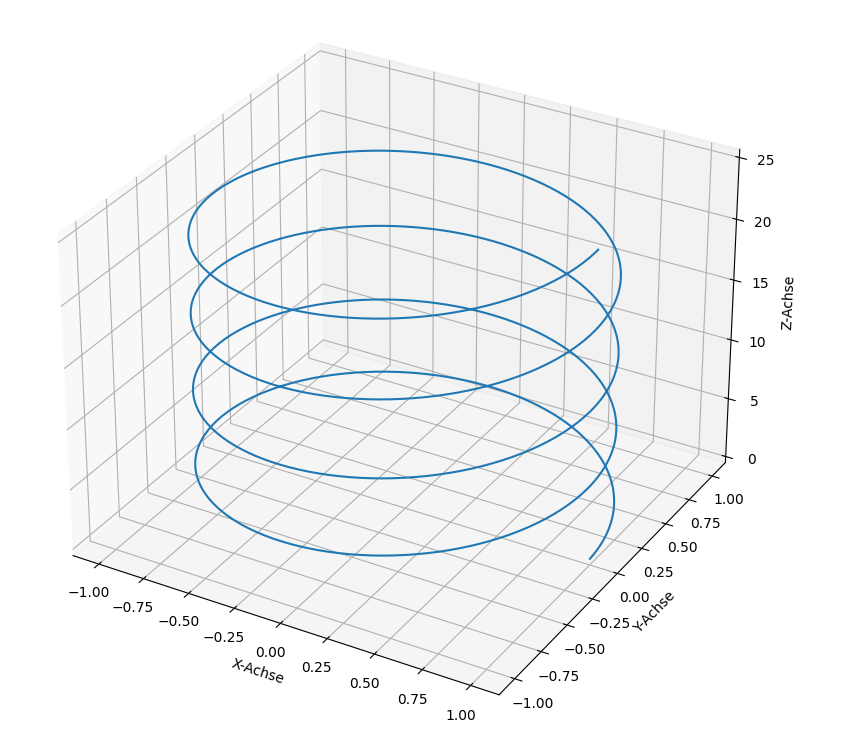
\includegraphics[scale = 0.3]{Bilder/Spirale_Kurven.png}
    \caption{Die Grafik visualsiert die Kurve $f(t)=(\cos(t),\sin(t),t)$}
\end{figure}}
\dfn{Geschwindigkeit}{Seien $I$ ein Intervall, und $f: I \rightarrow \mathbb{R}^n$ eine differenzierbare Kurve. Dann heisst der Vektor
$$
f^{\prime}(t)=\left(f_1^{\prime}(t), \ldots, f_n^{\prime}(t)\right)
$$
der Geschwindigkeitsvektor zum Zeitpunkt $t$.\newline
Seine Länge $\left\|f^{\prime}(t)\right\|$ heisst Geschwindigkeit zum Zeitpunkt $t$.\newline
Ist $f^{\prime}\left(t_0\right) \neq 0$ für ein $t_0$, so heisst
$$
\begin{aligned}
g: & \mathbb{R} \rightarrow \mathbb{R}^n \\
g(t)= & f\left(t_0\right)+t f^{\prime}\left(t_0\right)
\end{aligned}
$$
die Tangente an $f$ in $f\left(t_0\right)$.}
\dfn{Winkel}{Seien $f: I \rightarrow \mathbb{R}^n$ und $g: I \rightarrow \mathbb{R}^n$ zwei Kurven mit $f\left(t_1\right)=g\left(t_2\right)$. Sind die Geschwindigkeitsvektoren $f^{\prime}\left(t_1\right), g^{\prime}\left(t_2\right) \neq 0$, dann ist der Winkel $\Theta$ zwischen den Kurven im Punkt $f\left(t_1\right)=g\left(t_2\right)$ definiert durch
$$
\cos \Theta=\frac{\left\langle f^{\prime}\left(t_1\right), g^{\prime}\left(t_2\right)\right\rangle}{\left\|f^{\prime}\left(t_1\right)\right\|\left\|g^{\prime}\left(t_2\right)\right\|}
$$}

\ex{}{
    Sei $f(x)= \frac{1}{4}x^2$ und $g(x)=(x-1)^3$. Dann ist der Schnittpunkt 
    \begin{align*}
        \frac{1}{4}x^2&=(x-1)^3\\
        x&=2
    \end{align*}
    $$
    \frac{d}{d x}\left((x-1)^3\right)=3(x-1)^2=3 \text{ für } x =2 
    $$
    $$
\frac{d}{d x}\left(\frac{x^2}{4}\right)=\frac{x}{2}=1 \text{ für } x=2
$$
\begin{figure}[H]
    \centering
    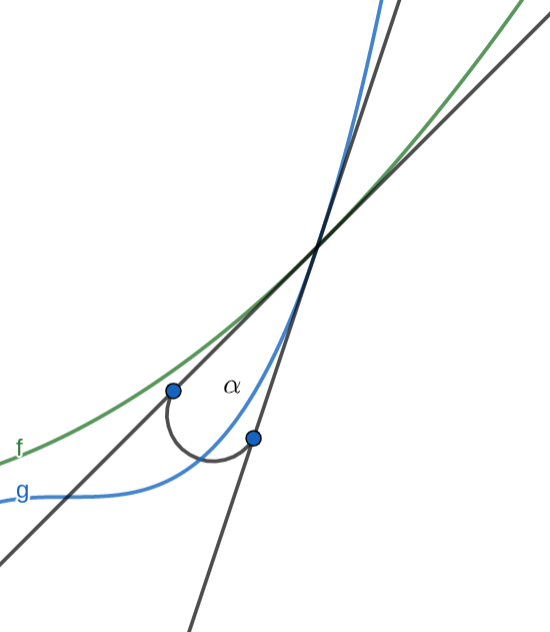
\includegraphics[scale = 0.3]{Bilder/AngleOf2Curves.png}
    \caption{Eine visuelle Vorstellung dieses Winkels, des Schnittpunktes zweier Funktionen $f$ und $g$, und wie er durch die Tangenten berechenbar ist.}
\end{figure}
}



















\chapter{Funktionen im $\mathbb{R}^n$}
\section{Krümmung}
\dfn{}{Sei $g:[0, L]$ eine zweimal steigt differenzierbare Kurve, parametrisiert nach Bogenlänge. Dann heißt
$$
T(s)=g^{\prime}(s)
$$
Tangentialvektor der Kurve,
$$
\kappa=\kappa(s)=\left\|T^{\prime}(s)\right\|_2 = \left|\frac{d\psi}{ds}\right|
$$
heißt Krümmung der Kurve im Punkt $g(s)$ und
$$
N(s)=\frac{T^{\prime}(s)}{\kappa(s)}
$$
heißt Normalenvektor (definiert, wenn $\kappa(s) \neq 0$ ), also
$$
T^{\prime}(s)=\kappa(s) N(s)
$$}
\nt{Da $g$ parametrisiert ist, ist $\|T\| = 1$.\newline
 $N(s)$ ist einfach nur die normierte Zweite Ableitung, folgt aus der Eigenschaft das $\|T\| = 1$.
\begin{align*}
     1 & = \langle T(s),T(s) \rangle\\
     \frac{d}{ds} 1 &= \frac{d}{ds}\langle T(s),T(s) \rangle\\
     0 &= \frac{d}{ds}\sum t_i^2\\
     0 &= 2\sum t_i\cdot t_i^{'}\\
     0 &= \langle T(s),T^{'}(s) \rangle\\
 \end{align*}
 }
\dfn{Krümmungskreis}{Für ebene Kurven ist der Kreis mit Mittelpunkt $g(s)+\frac{1}{\kappa} N(s)$ und Radius $r=\frac{1}{\kappa}$, der Kreis, der die Kurve $g(s)$ am besten approximiert. Wir nennen diesen Kreis den Krümmungskreis.}
\nt{Da $\|N(s)\|=1$ gibt $r\cdot N(s)$ exakt die Radius Länge. Je größer die Kurve gekrümmt ist, desto kleiner wird der Kreis, während desto flacher die Kurve ist der Kreis auch flacher wird und sich perfekt anähert.}

\section{Kurven in $\mathbb{R}^3$}
\dfn{}{Sei $g:[0, L] \rightarrow \mathbb{R}^3$ eine Kurve, die nach Bogenlänge parametrisiert ist. Dann ist $N \perp T$. Wir wählen nun $B \in \mathbb{R}^3$ so, dass
$$
(T, N, B)
$$
eine orientierte Orthonormalmatrix bilden.\newline
Der Vektor $B$ heißt Binormalenvektor und das Tripel $(T, N, B)$ heißt Fresnelsches Dreibein.}
\thm{}{Die Ableitung des Binormalenvektors $B(s)$ kann durch
$$
B^{\prime}(s)=-\tau(s) N(s)
$$
beschrieben werden, wobei $\tau(s)$ eine bestimmte Funktion $R \rightarrow R$ ist. Wir nennen $\tau(s)$ die Torsion der Kurve im Punkt $g(s)$.}
\nt{
    \begin{align*}
        B(s) &= T(s)\times N(s)\\
        \frac{d B(s)}{ds}&=\frac{d(T(s) \times N(s))}{ds}\\
        &=\frac{d T(s)}{ds}N(s) \times N(s)+T(s) \times \frac{d N(s)}{d s}\\
        &=\kappa N(s) \times N(s)+T(s) \times \frac{d N(s)}{d s}\\
        &= T(s)\times \frac{d N(s)}{ds}\\
        &\text{$T(s)\implies$ orthogonal zu $T(s)$}\\
        &\text{da $r(s)\cdot r^{'}(s) = 0$ für alle $r$ mit $\|r\|=1$, muss $\frac{dB(s)}{ds}$ orthogonal zu $B(s)$ sein }\\
        &= \tau N(s)
    \end{align*}}
\section*{Funktionen auf $\mathbb{R}^n$}
\dfn{}{Mit $f: D \subset \mathbb{R}^n \rightarrow \mathbb{R}$ ordnen wir jedem Element von $D \subset \mathbb{R}^n$ einen reellen Wert zu.
Die Menge $\Gamma_f:=\{(x, y) \in D \times \mathbb{R} \mid f(x)=y\}$ ist der Graph von $f$.}
\dfn{Niveaumenge}{Sei $f: D \rightarrow \mathbb{R}$ und $c \in \mathbb{R}$. Die Menge aller Punkte $x$ für die $f(x)=c$,
$$
N_c(f)=\{x \in D \mid f(x)=c\},
$$
heißt Niveaumenge von $f$ zum Niveau $c$.}
\nt{Man erhält den Contourplot durch mehrfaches plotten von verschiedenen Niveaumengen.}
\begin{figure}[H]
    \centering
    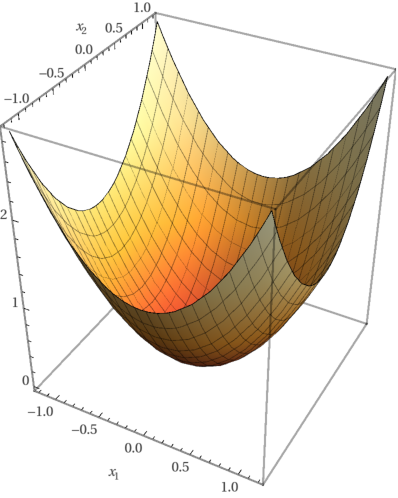
\includegraphics[scale = 1]{Bilder/F.pdf}
    \quad
    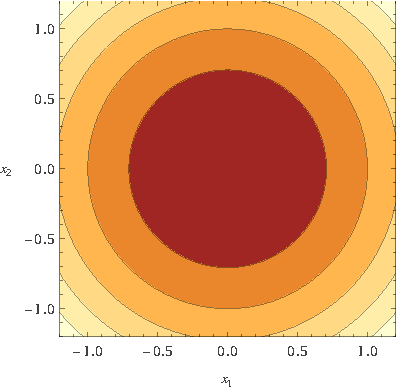
\includegraphics[]{Bilder/F_countour.pdf}
    \caption{Die Funktion $f(x_1, x_2) = x_1^2  +x_2^2$ und ihr Contourplot}
\end{figure}
\dfn{Offener und abgeschlossener Ball}{Sei $a \in \mathbb{R}^n$ und $r>0$. Dann ist die Menge
$$
B_r(a):=\left\{x \in \mathbb{R}^n \mid\|x-a\|_2<r\right\}
$$
ein offener Ball mit Radius $r$ und
$$
\overline{B_r(a)}:=\left\{x \in \mathbb{R}^n \mid\|x-a\|_2 \leq r\right\}
$$
ein abgeschlossener Ball mit Radius $r$.}
\dfn{Offen und abgeschlossen}{Sei $U \subset \mathbb{R}^n$ eine Teilmenge.\newline
$U$ heißt offen, falls $\forall a \in U: \exists \varepsilon>0$ so dass $B_{\varepsilon}(a) \subset U$.\newline
Eine Teilmenge $A \subset \mathbb{R}^n$ heißt abgeschlossen, wenn $\mathbb{R}^n \backslash A$ offen ist.}
\nt{$B_r(a)$ ist offen und $\overline{B_r(a)}$ ist abgeschlossen.}
\dfn{beschränkt und kompakt}{Eine Teilmenge $D \subset \mathbb{R}^n$ heißt beschränkt, wenn es ein $r>0$ gibt, so dass $D \subset B_r(0)$. Eine abgeschlossene und beschränkte Menge $K \subset \mathbb{R}^n$ heißt kompakt.}
\dfn{}{Sei $D \subset \mathbb{R}^n$ eine Teilmenge.
$$
\stackrel{\circ}{D}:=\left\{x \in \mathbb{R}^n \mid \exists \varepsilon>0: B_{\varepsilon}(x) \subset D\right\}
$$
ist die Menge der inneren Punkte von $D$. Mit
$$
\bar{D}:=\left\{x \in \mathbb{R}^n \mid B_{\varepsilon}(x) \cap D \neq \emptyset \forall \varepsilon>0\right\}
$$
bezeichnen wir den Abschluss von $D$. Der Rand von $D$ ist
$$
\partial D=\bar{D} \backslash \stackrel{\circ}{D}
$$}
\nt{noch keine Ahnung was ich dazu sagen soll :)}
\ex{}{$$
B_r(a) \text { ist der Abschluss von } B_r(a) \text { und } \partial B_r(a)=\left\{x \in \mathbb{R}^n \mid\|x-a\|_2=r\right\} \text { ist die Kugeloberfläche }
$$}
\section{Differentiation}
\dfn{stetig}{Sei $D \subset \mathbb{R}^n, f: D \rightarrow \mathbb{R}$ eine Funktion.
Die Funktion $f$ heißt stetig in $a \in D \subset \mathbb{R}^n$, wenn für alle $\varepsilon>0$ ein $\delta>0$ existiert, so dass
$$
|f(x)-f(a)|<\varepsilon \quad \forall x \in D
$$
mit $\|x-a\|_2<\delta$}
\thm{}{Summe, Produkte und Quotienten (falls definiert) stetiger Funktionen sind stetig.}
\dfn{Partiell differenzierbar}{Sei $f: U \rightarrow R, a=\left(a_1, \ldots, a_n\right) \in U$
Dann heißt $f$ in a partiell nach $x_i$ differenzierbar, wenn die Funktion in einer Variablen
$$
x_i \mapsto f\left(a_1, \ldots, a_{i-1}, x_i, a_{i+1}, \ldots, a_n\right)
$$
nach $x_i$ differenzierbar ist. Dann heißt
$$
\frac{\partial f}{\partial x_j}(a):=\lim _{h \rightarrow 0} \frac{f\left(a_1, \ldots, a_{i-1}, a_i+h, a_{i+1}, \ldots, a_n\right)-f\left(a_1, \ldots, a_{i-1}, a_i, a_{i+1}, \ldots, a_n\right)}{h}
$$
die partielle Ableitung von $f$ nach $x_i$.}
\nt{Die komplexe Version der Ableitung vom Ein-dimensionalem falls
$$
\frac{df}{dx}(x) = \lim_{h\to \infty}\frac{f(x+h)-f(x)}{h}
$$}
\dfn{Gradient}{Ist $f: U \rightarrow \mathbb{R}, U$ offen, in jedem Punkt nach allen Variablen partiell differenzierbar, dann heißt $U$ partiell differenzierbar auf $U$. Der Vektor
$$
\nabla f(a):=(\operatorname{grad} f)(a):=\left[\begin{array}{lll}
\frac{\partial f}{\partial x_1}(a) & \ldots & \frac{\partial f}{\partial x_n}(a)
\end{array}\right]
$$
heißt Gradient von $f$ im Punkt $a \in U$.}
\ex{}{Sei $f(x,y) = (x^2+y^2, x\cdot y^2)$. Dann ist 
\begin{align*}
    \nabla f(x,y)&=(\operatorname{grad} f)(x,y):=\left[\begin{array}{ll}
        \frac{\partial f}{\partial x}(x,y) ,& \frac{\partial f}{\partial y}(x,y)
        \end{array}\right]\\
        &=(2x,2xy)
\end{align*}
}
\dfn{Hesse-Matrix}{Die Matrix
$$
\operatorname{Hess}(f)=\left(\frac{\partial^2 f}{\partial x_i \partial x_j}\right)_{i j}=\left[\begin{array}{cccc}
\frac{\partial^2 f}{\partial x_1^2} &  \cdots & \frac{\partial^2 f}{\partial x_1 \partial x_n} \\
\vdots & & \vdots \\
\frac{\partial^2 f}{\partial x_n \partial x_1} & \cdots &\frac{\partial^2 f}{\partial x_n^2} 
\end{array}\right]
$$
heißt Hesse-Matrix.}
\thm{}{Sei $f: U \rightarrow \mathbb{R}$ zweimal stetig differenzierbar, dann gilt
$$
\frac{\partial^2 f}{\partial x_i \partial x_j}=\frac{\partial^2 f}{\partial x_j \partial x_i} .
$$
Das heißt unter diesen Voraussetzungen ist die Hesse-Matrix symmetrisch.}
\ex{}{Sei $f(x,y)=\sqrt{x^2(1-y)}$, dann ist 
$$\operatorname{Hess}(f) = \left[\begin{array}{ccc}
    6x\cdot y^2 & 4x\cdot y^3\cdot z^2\cdot c^2 & 0\\
    4x\cdot y^3\cdot z^2 &  
\end{array}\right]$$
}





\chapter{Taylorformel und Extremstellen}
\section{Kettenregel}
\dfn{}{Sei $ U \subset \mathbb{R}^n$ offen, $f: U \rightarrow \mathbb{R}^m$ $f(u) \subset V \subset \mathbb{R}^m$ und $V$ offen, sowie $g: V \rightarrow \mathbb{R}$ und $h=g \circ f$ 
Die Koordinaten in $U$ bezeichnen wir mit $x_i$, die in $V$ mit $x_j$. Dann gilt
$$
\frac{\partial h}{\partial x_i}(x)=\sum_{j=1}^m \frac{\partial g}{\partial y_j}\left(f(x)\right) \frac{\partial f_j}{\partial x_i}(x)
$$}
\nt{Die Kettenregel lässt sich über herleiten durch nutzen der Taylor-Entwicklung Erster Ordnung:\newline
Seien $f,g,h$ definiert wie oben, dann ist
\begin{equation}\label{eq:1}    
g(y) \approx g(f(x))+\sum_{j=1}^m \frac{\partial g}{\partial y_j}(f(x))\left(y_j-f_j(x)\right).
\end{equation}
Für $f$ in der Nähe von $x$ erhält man:
$$
f_i(x+\Delta x) \approx f_i(x)+\sum_{k=1}^n \frac{\partial f_i}{\partial x_k}(x) \Delta x_k
$$
Da Eq:\ref*{eq:1} $h$ beschreibt und man an der Entwicklungsstelle $h(x+\Delta x)$ interessiert sind, setzt  man $y = f(x+\Delta x)$ in die Taylor-Entwicklung von $g$ ein
\begin{align*}
h(x+\Delta x) &\approx g(f(x+\Delta x))+\sum_{j=1}^m \frac{\partial g}{\partial y_j}(f(x))\left(f_j(x+\Delta x)-f_j(x)\right)\\
h(x)+\Delta h(x)&\approx g(f(x))+\sum_{j=1}^m \frac{\partial g}{\partial y_j}(f(x))\left(\sum_{k=1}^n \frac{\partial f_j}{\partial x_k}(x) \Delta x_k\right)\\
\Delta h(x) &\approx \sum_{j=1}^m \frac{\partial g}{\partial y_j}(f(x))\left(\sum_{k=1}^n \frac{\partial f_j}{\partial x_k}(x) \Delta x_k\right)\quad \text{ da $h(x)=g(f(x))$}\\
\frac{\Delta h(x)}{\Delta x_i} &\approx \sum_{j=1}^m \frac{\partial g}{\partial y_j}(f(x))\left(\sum_{k=1}^n \frac{\partial f_j}{\partial x_k}(x) \frac{\Delta x_k}{\Delta x_i}\right)\\
\frac{\partial h}{\partial x_i}(x)=\lim _{\Delta x_i \rightarrow 0} \frac{\Delta h(x)}{\Delta x_i} &= \sum_{j=1}^m \frac{\partial g}{\partial y_j}(f(x)) \frac{\partial f_j}{\partial x_i}(x)\quad \text{ da $\frac{\Delta x_k}{\Delta x_i}$ wird 0 für alle $k\neq i$}\\
\end{align*}
}
\ex{}{Sei $f(r,\phi) = (r\cdot \cos(\phi),r\cdot \sin(\phi))$, dann ist 
$$J_f = \operatorname*{D}f = \left[\begin{array}{cc}
    \cos(\phi) & -r\cdot \sin(\phi)\\
    \sin(\phi) & r\cdot \cos(\phi)
\end{array}\right]$$
Sei $g(x,y) = x^2+ y^2$, dann ist $\operatorname*{D}g = (2x,2y)$.\newline
Sei $h = g\circ f$, dann ist gilt
$$h(r,\phi) = (r\cdot \cos(\phi))^2+(r\cdot \sin(\phi))^2 = r^2 $$
Von hier ist leicht zu sehen, dass 
$$\frac{\partial h}{\partial r} = 2r\quad \frac{\partial h}{\partial \phi} = 0$$
\begin{align*}
    \operatorname*{D} h(r,\phi) &= \operatorname*{D}g(f(r,\phi))\cdot \operatorname*{D}f\\
    &= (2 r \cos f, 2 r \sin \phi) \cdot \operatorname*{D} f(r, \phi) \\
    & = (2 r, 0)
\end{align*}
Es kann auch über die Formel berechnet werden
\begin{align*}
    \frac{\partial h}{\partial r}(r,\phi) &= \frac{\partial g}{\partial x}(f(r,\phi))\frac{\partial f_1}{\partial r}(r,\phi)+ 
    \frac{\partial g}{\partial y}(f(r,\phi))\frac{\partial f_2}{\partial r}(r,\phi)\\
    &= 2\cdot (r\cos(\phi))\cos(\phi)+2\cdot(r\sin(\phi))\sin(\phi)\\
    &=2r
\end{align*}
\begin{align*}
    \frac{\partial h}{\partial \phi}(r,\phi) &= \frac{\partial g}{\partial x}(f(r,\phi))\frac{\partial f_1}{\partial \phi}(r,\phi)+ 
    \frac{\partial g}{\partial y}(f(r,\phi))\frac{\partial f_2}{\partial \phi}(r,\phi)\\
    &=2\cdot(r\cdot \cos(\phi))\cdot(-r\sin(\phi))+2\cdot(r\cdot \sin(\phi))\cdot(r\cos(\phi))\\
    &=0
\end{align*}
Man erhält das gleiche Ergebnis
    }











\section{Richtungsableitungen}
\dfn{}{Sei $U \subset \mathbb{R}^n$ offen und $f: U \rightarrow \mathbb{R}, a \in U$ und $v \in \mathbb{R}^n$ mit $\|v\|=1$, Dann heißt
$$\left(D_v f\right)(a)=\lim _{h \rightarrow 0} \frac{f(a+h \cdot v)-f(a)}{h}$$
Richtungsableitung von $f$ in Richtung $v$.}
\thm{}{Sei $f: U \rightarrow \mathbb{R}, U \in \mathbb{R}^n$ offen, total und differenzierbar in $a$. Dann gilt
$$
(D_v f)(a)=\langle(\operatorname{grad} f)(a), v\rangle \text {. }
$$
Insbesondere: Für $v\in g^{n-1}:=\left\{v e \mathbb{R}^n \mid\|v\|=1\right\}$ ist die Richtungsableitung maximal genau dann, wenn de fradiar (gradf) (a) in die Gluide Ridehueg wie V zeigt}
\section{Taylorpolynome}
\dfn{Multiindex}{$\alpha=\left(\alpha_1, \ldots, \alpha_n\right) \in \mathbb{N}^n$ nennen wir einen Multiindex.
$|\alpha|=\alpha_1+\ldots+\alpha_n$ heißt Totalgrad von $\alpha$. Wir setzen $x^\alpha=x_1^{\alpha_1} x_n^{\alpha_n}$ Damnn bezeichnet
$$
\operatorname*{D}^\alpha f:=\frac{\partial^{|\alpha|} f}{\partial x^\alpha}=\frac{\partial^{|\alpha|} f}{\partial x_1^{\alpha_1} \ldots \partial x_n^{\alpha_n}}
$$
Die $\alpha$-te partielle Ableitung.}
\ex{}{\begin{align*}
    & \alpha=(1,2,3) \quad\left|\alpha\right|=1+2+3=6 \\
    & \operatorname*{D}^\alpha f=\frac{\partial^6 f}{\partial x_1 \partial x_2^2 \partial x_3^3}
    \end{align*}}
\dfn{Taylorpolynome}{Sei $U \subset \mathbb{R}^n$ offen, $a \in U$. sei $f: u \rightarrow \mathbb{R}$ $k$-mal stetig partiell differenzierbar. Dann heißt das polynom
$$
\sum_{|\alpha| \leq k} \frac{\partial|\alpha| f}{\partial x|\alpha|}(a) \cdot \frac{(x-a)^\alpha}{\alpha !}
$$
das Taylorpolynom $k$-ter Ordnung vou $f$ in a.}
\nt{Eine hübsche andere Formel für den Fall $U\subset \mathbb{R}^2$ und $f:U\to \mathbb{R}$, ist über die Summe der binomischen Formeln:
$$f(x) = f+\sum_{i=1}^k\frac{1}{i!}\left(\frac{\partial f}{\partial x}(x-a)+\frac{\partial f}{\partial y}(y-a)\right)^i$$ mit $f$ evaluiert an der Stelle $a$. Der Zussamenhang folgt aus der Beziehung zum Binomialkoeffizienten, da man bei $\alpha$ $k$ Elemente aus $n$ auswählt.}
\ex{}{
Sei $f(x,y) = e^{-x^2-y^2}$ und der Entwicklungspunkt $a=(1,1)$, dann sind 
$$
\frac{\partial f}{\partial x}=-2 x e^{-x^2-y^2}\quad 
\frac{\partial f}{\partial y}=-2 y e^{-x^2-y^2}
$$
Die ersten partiellen Ableitungen und 
$$
\frac{\partial^2 f}{\partial x^2}=\left(4 x^2-2\right) e^{-x^2-y^2} \quad \frac{\partial^2 f}{\partial x\partial y}=4 x y e^{-x^2-y^2}\quad
\frac{\partial^2f}{\partial y^2}=\left(4 y^2-2\right) e^{-x^2-y^2}
$$
Daraus folgt das Das Taylorpolynom erster Ordnung 
$$
f(x) = f(a) + \frac{\partial f}{\partial x}(a)\cdot(x-a) + \frac{\partial f}{\partial y}(a)\cdot (y-a) = 1
$$
Das Taylorpolynom 2-ter Ordnung ist 
\begin{align*}
    f(x) &= f(a) + \frac{\partial f}{\partial x}(a)\cdot(x-a) + \frac{\partial f}{\partial y}(a)\cdot (y-a)\\
    &+ \frac{1}{2}\left(\frac{\partial^2 f}{\partial x^2}(a)\cdot (x-a)^2+\frac{\partial^2 f}{\partial x\partial y}(a)\cdot (x-a)(y-a)
    +\frac{\partial^2f}{\partial y^2}(a)\cdot (y-a)^2\right)\\
    &= 1-x^2-y^2
\end{align*}
\begin{figure}[H]
    \centering
    \includegraphics*[scale=0.15]{Bilder/Taylopolynome.png}
    \caption{Die Funktion $f(x, y) = e^{-x^2 - y^2}$ und die Taylorpolynome erster und zweiter Ordnung um den Entwicklungspunkt $(0,0)$.}
\end{figure}
}
\section{Extrempunkte, Maxima, Minima}
\dfn{}{Ser $f: u \rightarrow \mathbb{R}, U \subset \mathbb{R}^n$.
$f$ hat ein lokales 
(lokales Muimun), wenn ein Ball
$Br (a) \subset U$ existiert, so dass $\left.f\right|_{B_r(a)}$
in $a$ das Maximum (Minimun) hat.\newline
$f$ hat ein lokales Extrema, wenn eine der beiden Bediengungen eintritt.}
\mlenma{}{Die Matrix $A=A^{\top} \in \mathbb{R}^{n\times n}$ ist positiv definit, falls
\begin{align*}
    &x^{\top} A x>0 \quad \forall x \in \mathbb{R}^n \backslash\{0\} \text {. }\\
    &\iff \text{ alle Eigenwerte der Matrix  $> 0$ sind}
\end{align*}
}
\thm{Minima und Maxima}{Sei $U \subset \mathbb{R}^k$ offen: $f: U \rightarrow \mathbb{R}$ zweimal stetig partiell differenzierbar
\begin{itemize}
    \item[1] Notwendig dafür, dass $f$ in $a \in U$ ein lokales Extrema hat, ist dass
    $$
    \frac{\partial f}{\partial x_1}(a)=\ldots=\frac{\partial f}{\partial x_n}(a)=0
    $$Ist die notwendige Bedingung erfüllt, dann ist hinreichend für ein lokales Minimum, dass die Matrix
    $$
    A=\operatorname{Hess}(f)(a)=\left(\frac{\partial^2 f}{\partial x_i \partial x_j}(a)\right)_{i j}
    $$
    positiv definit ist. Ist $A$ negativ definit dann liegt ein lokales Maximun vor.
\end{itemize} 
}
\ex{}{
    $$
\begin{aligned}
& f(x, y)=x^2+y^2 \quad \frac{\partial f}{\partial x}=2 x=0 \\
& \frac{\partial f}{\partial y}=2 y=0
\end{aligned}
$$
$\Rightarrow(0,0)$ ist der einzige Kandidat für ein lokales Extrema
$$
\operatorname*{Hess}(f)(a)=\left[\begin{array}{ll}
2 & 0 \\
0 & 2
\end{array}\right]>0
$$
Folglich hat die Funktion in (0,0) ein lokales Minima.
}
\chapter{Hyperflächen und Satz über implizite Funktionen}
\section{Hyperflächen}
\dfn{}{Sei $f:\mathbb{R}^n \to \mathbb{R}$ eine differenzierbare Funktion. Dann heißt ihre Nullstellenmenge
$$N(f):=N_0(f)=\{a\in \mathbb{R}^n\mid f(a)=0\}$$
die durch $f$ definierte Hyperfläche.
}
\ex{}{$x^2+y^2+z^2-1 = 0$  ist eine Kugel, siehe abb. \ref*{fig:kreis}}
\begin{figure}[H]
    \centering
    \includegraphics*{Bilder/Kugel.pdf}
    \caption{Eine 3-dimensionale Kugel mit dem Radius 1}
    \label{fig:kreis}
\end{figure}
\section{Tangentialraum}
\dfn{}{Sei $X=N(f)$, $f$ stetig differenzierbar, eine Hyperfläche und $a \in X$. Dann ist
$$
f(x)=f(a)+\sum_{j=1}^n \frac{\partial f}{\partial x_j}(a)\left(x_j-a_j\right)+\sigma(\|x-a\|)
$$
die erste Taylorformel (zum Landau Syubol $\sigma(1 )$)
\footnote{Ich denke das hier einfach der Rest Term eines Taylorpolynoms gemeint ist und das dieser langsamer wächst als $\|\|x-a\|\|\iff o(\|\|x-a\|\|)$}, so heißt
$$
T_a x=\left\{x \in \mathbb{R}^n \mid \sum_{j=1}^n \frac{\partial f}{\partial x_j}(a)\left(x_j-a\right)=0\right\}
$$
der Tangentialraum von $X$ im Punkt $a$}
\cor{Glatt oder Singulär}{$T_a X$ ist der zu $\operatorname{grad} f(a)$ orthogonale Untervektorraum:
$$
\left\{x \in \mathbb{R}^n \mid\langle\operatorname{grad} f(a), x\rangle=0\right\}
$$
Falls $\operatorname{grad} f(a) \neq 0$, ist $T_a X$ eine Hyperebene und $x$ ist glatt in a. Andernfalls ist $T_a X$ der gesamte Raum und $x$ ist singulär in a.

In dieser überarbeiteten Formulierung beschreibt der Tangentialraum $T_a X$ den Untervektorraum, der orthogonal zum Gradienten von f an der Stelle a ist. Der Gradient von f, oft als $\operatorname{grad} f(a)$ bezeichnet, gibt die Richtung des steilsten Anstiegs der Funktion f an der Stelle a an.

Wenn der Gradient von f an der Stelle a ungleich Null ist, bildet der Tangentialraum eine Hyperebene, und die Funktion ist glatt (d. h. differenzierbar) an der Stelle a. Wenn der Gradient jedoch gleich Null ist, entspricht der Tangentialraum dem gesamten Raum, und die Funktion hat an der Stelle a einen singulären Punkt (d. h. sie ist möglicherweise nicht differenzierbar oder hat einen kritischen Punkt).}
\section{Satz über implizite Funktionen}
\dfn{}{Sei $U \subset \mathbb{R}^n$ offen, $f: U \rightarrow \mathbb{R}$ mal stetig differenzierbar und
\begin{equation}
a=\left(a_1, \ldots, a_{n-1}, a_n\right) \in N(f),
\end{equation}
gilt $\frac{\partial f}{\partial x_n}(a) \neq 0$, dann existieren offene Umgebungen $V^{\prime} \subset \mathbb{R}^{n-1}$ von $\left(a_1, \ldots, a_{n-1}\right)=: a^{\prime}$ und $V^{\prime \prime} \subset \mathbb{R}$ von $a_n=: a^{\prime \prime}$ mit $V^{\prime} \times V^{\prime \prime} \subset U$ und es existiert eine Funktion $g: V^{\prime} \rightarrow V^{\prime \prime}$ und $g\left(a^{\prime}\right)=a^{\prime \prime}$ und
\begin{enumerate}
    \item $f\left(x_1, \ldots, x_{n-1}, g\left(x_1, \ldots, x_{n-1}\right)\right)=0$ $\forall x^{\prime}=\left(x_1, \ldots, x_{n-1}\right) \in V^{\prime}$ und
    \item $\forall\left(x^{\prime}, x^{\prime \prime}\right) \in\left(V^{\prime} \times V^{\prime \prime}\right) \cap N(f)$ gilt $x^{\prime \prime}=x_n=g\left(x^{\prime}\right)$.
\end{enumerate}
$g$ ist lokal stetig differenzierbar und
\begin{equation}
\frac{\partial g}{\partial x_i}\left(a^{\prime}\right)=-\frac{\partial f}{\partial x_i}(a) / \frac{\partial f}{\partial x_n}(a) \quad \text{für } i=1, \ldots, n-1 .
\end{equation}}
\nt{Grundlegend besagt der Satz, dass wenn eine Gleichung in der Form $f(x_1, x_2, \ldots, x_n) = 0$ eine Funktion implizit definiert und bestimmte Regularitätsbedingungen erfüllt sind, dann kann man die Ableitungen dieser impliziten Funktion berechnen, ohne sie explizit zu lösen.}
\chapter{Integration im $\mathbb{R}^n$}
\section{Doppelintegral}
\dfn{}{Der Grenzwert
$$
\lim_{\substack{h \to \infty \\ \Delta A_k \to 0}} \sum_{k=1}^h f(x_k, y_k) \Delta A_k
$$
wird (falls er existiert) als Doppelintegral bezeichnet und durch 
$$
\iint_A f(x, y) dA
$$
gekennzeichnet.}
\nt{Angenommen, die Fläche A ist in M Reihen und N Spalten unterteilt, 
wobei die Breite der iten Spalte $\Delta \mathrm{x}_{-}$i und die Höhe der j-ten Reihe $\Delta \mathrm{y}_{-}$j ist.\newline
Die Fläche der kleinen rechteckigen Teilfläche an der Position (i, j) ist dann $\Delta \mathrm{A}_{-} \mathrm{ij}=\Delta \mathrm{x}_{-} \mathrm{i} \Delta \mathrm{y}_{-} \mathrm{j}$.
$$S=\sum_{i=1}^M \sum_{j=1}^N f\left(x_{i j}, y_{i j}\right) \Delta A_{i j}$$
Der Grenzwert dieser Flächen ist dann das Integral, in Abb: \ref{fig:Doppelintegral} ist eine solche Teilfäche zu sehen
$$
\iint_A f(x, y) d A=\lim _{\substack{\Delta x_i, \Delta y_j \rightarrow 0 \\ M, N \rightarrow \infty}} \sum_{i=1}^M \sum_{j=1}^N f\left(x_{i j}, y_{i j}\right) \Delta A_{i j}
$$
Ich finde diese Formel etwas intuitiver, da klar ist was $k$ und $\delta A_k$ sind. 
\newline
In Bezug auf ihre Integrationsgrenzen ergibt sich 
$$
\iint_A f(x, y) d A=\int_a^b \int_c^d f(x, y) d y d x
$$
    \begin{figure}[H]
        \centering
        \includegraphics*[scale=0.1]{Bilder/Surface_integral1.png}
        \caption{
            Eine Illustration eines einzelnen Oberflächenelements. Diese Elemente werden durch den Integrierungsprozess unendlich klein gemacht, um sich der Oberfläche anzunähern.}
        \label{fig:Doppelintegral}
        \end{figure}
        $$
        \iint_A f(x, y) d t=\int_{x=a}^b \underbrace{\int_{y=f_u(x)}^{f_0(x)} f(x, y) d y}_{\text {Inneres Integral }} d x
        $$
        Das innere Integral wird für unendlcih viele infintisemal wenig aus einanderliegernde $x$ berechnet.
        Dann werden all diese Integrale, genau wie bei einem einfachen Integral Funktionswerte, integriert.
        \newline
        In der Abb \ref*{fig:Doppelintegral_innere} ist bspw. das innere Integral für $x=0$ zu sehen.
    \begin{figure}[H]
        \centering
        \includegraphics*[scale=0.5]{Bilder/DoppelIntegralInnere.png}
        \caption{
            Die Funktion $f(x,y)=x^2+y^2$ und eine herausgeschnittene Scheibe $\int f(0,y)dy$}
        \label{fig:Doppelintegral_innere}
        \end{figure}        
}
\section{Berechnung eines Doppelintegrals unter Verwendung kartesischer Koordinaten}
\nt{\begin{itemize}
    \item Ein Doppelintegral wird von innen nach außen integriert, d.h. zuerst bezüglich der Variablen $y$ und dann bezüglich der Variablen $x$. Die Integrationsgrenzen des inneren Integrals sind dabei von $x$ abhängige Funktionen, während die des äußeren Integrals konstant oder von einer anderen Variablen abhängig sein können.
    \item -Die Reihenfolge der Integration ist normalerweise durch die Reihenfolge der Differentiale im Doppelintegral festgelegt. Sie sind jedoch austauschbar, wenn alle Integrationsgrenzen konstant sind (rechteckiges Integrationsgebiet).
\end{itemize}
}
\ex{}{
$$
B=\left\{(x, y): x^2+y^2 \leqslant r^2 ; x \geqslant 0, y \geqslant 0,r \in \mathbb{R}\right\}
$$
Es soll das Doppelintegral 
$$
\iint_B x \cdot y d B
$$ berechnet werden.
\begin{figure}[H]
    \centering
    \includegraphics*[scale=0.5]{Bilder/Kreis_Surface_Integral.png}
    \caption{
        Die Funktion $f(x,y)=x\cdot y$ für die Menge $B$}
    \label{fig:Kugel_Doppelintegral_Surface}
    \end{figure}  
In Abb. \ref*{fig:Kugel_Doppelintegral_Surface} ist die Funktion zu sehen, das Surface-Integral berechnet das Volumen unter dieser Funktion.
$$
\begin{aligned}
& B: a=0, b=R \\
& f_u(x)=0, f_0(x)=\sqrt{R^2-x^2} \\
& \iint_B x y d B=\int_0^R\left[\int_0^{\sqrt{R^2-x^2}} x y d y\right] d x \\
& =\left.\int_0^R x\cdot \frac{y^2}{2}\right|_0 ^{\sqrt{R^2-x^2}} d x \\
& =\int_0^R x\left(\frac{R^2-x^2}{2}\right) d x \\
& =\int_0^R \frac{R^2 x}{2}-\frac{x^3}{2} d x \\
& =\left[\frac{R^2 x^2}{4}-\frac{x^4}{8}\right]_0^R=\frac{R^4}{4}-\frac{R^4}{8} \\
& =\frac{R^4}{8} \\
&
\end{aligned}
$$
}
\nt{Beim Übergang von kartesischen Koordinaten $(x, y)$ zu Polarkoordinaten $(r, \varphi$ gelten die Transformationsgleichungen:
\begin{equation}
\begin{aligned}
x &= r \cos \varphi \\
y &= r \sin \varphi \\
dA &= r \, dr \, d\varphi
\end{aligned}
\end{equation}
Doppelintegral in Polarkoordinaten:
\begin{equation}
\iint_A f(x, y) \, dA = \int_{\varphi=\varphi_1}^{\varphi_2} \int_{r=r_i(\varphi)}^{r_a(\varphi)} f\left(r \cos \varphi, r \sin \varphi\right) \, r \, dr \, d\varphi
\end{equation}
\begin{enumerate}
    \item Innere Integration nach $r$ (Radialkoordinate)
    \item Äußere Integration nach $\varphi$
\end{enumerate}
Wir erhalten
$$
\begin{aligned}
\iint_B x y d B & =\int_0^{\pi / 2}\left[\int_0^R r \cos \varphi r \sin \varphi r d r\right] d \varphi \\
& =\int_0^R \left[\int_0^{\frac{\pi}{2}} r^3\cos \varphi \sin \varphi d \varphi\right] d r \\
& =\int_0^R r^3 \frac{1}{2}\left[\sin ^2 \varphi\right]_0^{\frac{\pi}{2}} d r \\
& =\frac{1}{2} \int_0^R r^3 d r=\frac{R^4}{8}
\end{aligned}
$$
}


\section{Transformation der Variablen}
\dfn{}{
    \begin{itemize}
        \item Durch die Funktion
        $$
        \begin{aligned}
        & x=\varphi(\tilde{x}, \tilde{y}) \\
        & y=\psi(\tilde{x}, \tilde{y})
        \end{aligned}
        $$
        werde der Bereich $\widetilde{\beta}$ der $\tilde{x}-\tilde{y}$-Ebene mit stückweise glattem Rand eineindeutig auf den Bereich $B$ der $x-y$-Ebene abgebildet.
        \item $x=\varphi(x, \tilde{y}), y-\varphi(x, \tilde{y})$ und ihre partiellen Ableitungen erster ordnung seien stetig in $\widetilde{B}$
        \item Im Inneren von $\widetilde{B}$ gelte für die Funktional determinante
        $$
        \operatorname{det}\left[\begin{array}{cc}
        \varphi_{\tilde{x}}\left(\tilde{x}, \tilde{y}\right) & \varphi_{\tilde{y}}(\tilde{x}, \tilde{y}) \\
        \psi_{\tilde{x}}(\tilde{x}, \tilde{y}) & \psi_{\tilde{y}}\left(\tilde{x}, \tilde{y}\right)
        \end{array}\right] \neq 0
        $$
        \item Ist dann die Funktion in $f(x,y)$ in $B$ stetig, so gilt $$
        \iint_B f(x, y) d B=\iint_{\tilde{B}} f\left(\varphi\left(\tilde{x}, \tilde{y}\right), \psi\left(\tilde{x}, \tilde{y}\right)\right) \operatorname{det}\left[\begin{array}{cc}
        \varphi_{\tilde{x}} &\varphi_{\tilde{y}} \\
        \psi_{\tilde{x}} &\psi_{\tilde{y}}
        \end{array}\right] d \tilde{B}
        $$
    \end{itemize}
}
\ex{}{Viertelkreis $\iint_B x y d B$
$$
B=\left\{(x, y): x^2+y^2 \leqslant R^2, x \geqslant 0, y \geqslant 0\right\}
$$
Transformation 
\begin{align*}
&x=r \cos \varphi \quad 0 \leqslant r \leqslant R\\
&y=r \sin \varphi \quad 0 \leqslant \varphi \leqslant \frac{\pi}{2}
\end{align*}
Zuordnung ist eineindeutig.
$$
\begin{aligned}
& x=\varphi(\tilde{x}, \tilde{y})=\varphi(r, \varphi)=r \cos \varphi \\
& y=\psi(\tilde{x}, \tilde{y})=\psi(r, \varphi)=r \sin \varphi
\end{aligned}
$$
$\varphi \psi$ sind stetig
$$
\begin{aligned}
& \varphi_r=\cos \varphi \quad \varphi_{\varphi}=-r \sin \varphi \\
& \psi_r=\sin \varphi \quad \psi_{\psi}=r \cos \varphi \\
&
\end{aligned}
$$
Funktional determinante
$$
\begin{aligned}
\operatorname{det}\left[\begin{array}{cc}
\varphi_r & \varphi_\varphi \\
\psi_r & \psi_\psi
\end{array}\right] & =\operatorname{det}\left[\begin{array}{cc}
\cos \varphi & -r \sin \varphi \\
\sin \varphi & r \cos \varphi
\end{array}\right] \\
& =r \cos ^2 \varphi+r \sin ^2 \varphi \\
& =r
\end{aligned}
$$
ist $\neq 0$ im Inneren von $\widetilde{B}$\newline
$\implies$ Transformationssatz ist anwendbar.}

\section{Rechenregeln für Integrale}
\dfn{}{\textbf{Additivität:}\newline
sind $f,g$ zwei integrierbare Funktionen, so gilt
$$
 \iint_B(f(x, y)+g(x, y)) d B =\int_B f(x, y) d B+\int_B g(x, y) d B
$$
\textbf{Additivität bzgl. der Bereiche:}\newline
Seien $B_1, B_2$ zwei Bereiche ohne gemeinsame innere Punkte, so gilt
$$
\iint_{B, \cup B_2} f(x, y) d B=\int_{B_1} f(x, y) d B+\iint_{B_2} f(x, y) d B
$$
\textbf{Konstanter Faktor:}\newline
Ist $k$ eine reele Zahl, so gilt
$$
\iint_B k f(x, y) d B=k \iint_B f(x, y) d B
$$
\textbf{Monotonie:}
Ist für jeden Punkt $(x, y) \in B$ $f(x, y) \leq g(x, y)$, so gilt
$$
\iint_B f(x, y) d B \leq \iint_B g(x, y) d B
$$
\textbf{Abschätzung:} Ist $f$ über $B$ integrierbar, so auch $|f|$ so gilt
$$
\left|\iint_B f(x, y) d B\right| \leqslant \iint_B|f(x, y)| d B
$$
\textbf{Eingrenzung:}\newline
Ist $m$ die untere, $M$ die obere grenze von $f$ in $B(m \leqslant M)$ und ist $|B|$ der Flächeninhalt von $B$, so gilt
$$
m|B|=\iint_R f(x, y) d B \leq M|B|
$$
\textbf{Mittelwertsatz:}
Wenn $f$ auf $B$ stetig ist, so existiert auf $B$ mindestens eine Stelle $(\xi, \eta)$ mit
$$
\iint_B f(x, y) d B=f(\xi, \eta)|B|
$$
}
\section{Dreifach-Integrale}
\dfn{}{Der Grenzwert
$$
\lim _{\substack{\Delta v_k \rightarrow 0}} \sum_{k=1}^{\infty} f\left(x_k, y_k, z_k\right) \Delta v_k
$$
wird (falls er existiert) alo Dreifach-Integral bezeichnet und duch das Symbol
$$
\iiint_V f(x, y, z) d V
$$
gekennzeichnet.}
\ex{}{Wenn $f:\mathbb{R}^3\to \mathbb{R}$ ist diese sehr schwer vorstellbar und vorallem nicht visualisierbar.\newline
Da der Funktionswert $f(x,y,z)$ nicht mehr eine Koordinate im kartesischen Koordinatensystem darstellt sondern eine gewisse Eigenschaft des Punktes $(x,y,z)$.\newline
In vielen Anwendungen wie in der Physik, könnte dies aber ausgenutzt werden. Sei 
$$
B=\{(x,y,z)\in\mathbb{R}^3\mid x^2+y^2+z^2 = 1\wedge x\geq 0 \wedge y\geq 0 \wedge z\geq 0 \}
$$
\begin{center}
    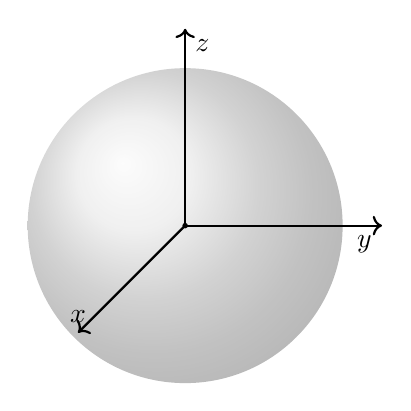
\begin{tikzpicture}
        % Kugel zeichnen
        \shade[ball color = gray!40, opacity = 0.4] (0,0) circle (2cm);
        \fill[fill=black] (0,0) circle (1pt);
        % Achsen zeichnen
        \draw[thick,->] (0, 0) -- (2.5, 0) node[anchor=north east]{$y$};
        \draw[thick,->] (0, 0) -- (0, 2.5) node[anchor=north west]{$z$};
        \draw[thick,->] (0, 0) -- (0,0,3.533) node[anchor=south]{$x$};
    \end{tikzpicture}
\end{center}

Dann ist der Körper die Kugel und $f(x,y,z)$ kann jetzt eine Eigenschaft über jeden der inneren Punkt beschreiben,
bspw. die Dichte an dieser Stelle und dann wäre das Dreifachintegral gerade die Masse dieser Kugel.\newline
An diesem Beispiel lässt sich auch sehr gut die Formel vorstellen, man Teilt die Kugel in unendlich viele infintisemal $\Delta A = dx\cdot dy\cdot dz$ große Stücke
und berechnet für diese die Dichte und summiert sie dann alle auf. In Abbildung \ref*{fig:Kugel_approximiert} ist dies versuchsweise dargestellt.
\begin{figure}[H]
    \centering
    \includegraphics*[scale=0.3]{Bilder/KugelApproximiert.png}
    \caption{Eine Kugel dargestellt als eine Menge von kleinen Würfeln}
    \label{fig:Kugel_approximiert}
    \end{figure}  
Der Grenzwert dieser Flächen ist dann das Integral
$$
\iiint_A f(x, y,z) d A=\lim _{\substack{\Delta x, \Delta y,\Delta z \rightarrow 0 \\ M, N,L \rightarrow \infty}} \sum_{i=1}^M \sum_{j=1}^N \sum_{k=1}^L f\left(x_{i j k}, y_{i j k},z_{ijk}\right) \Delta A_{i j k}
$$
Der Für uns aber häufig interresante Fall ist wenn $f(x,y,z)=1$, weil dann 
$$
\iiint_A f(x, y,z) d A
$$
gleich dem Volumen des Körpers ist.
}
\thm{Transformation von Variablen}{Die Voraussetzungen seien hier für Transformationsfunktionen 
$x=\varphi(\tilde{x}, \tilde{y}, \tilde{z}),y=\psi(x, \tilde{y}, \tilde{z}), z=\chi(\tilde{x}, \tilde{y}, \tilde{z})$ die selben wie im 2-dimensionalem. 
Ist dann im Inneren des Bereiches $V$ die Funktional-deternmiante
$$
\operatorname{det}\underbrace{\left[\begin{array}{lll}
\frac{\partial \varphi}{\partial \tilde{x}} & \frac{\partial \varphi}{\partial \tilde{y}} & \frac{\partial  \varphi}{\partial \tilde{z}} \\
\frac{\partial \psi}{\partial \tilde{x}} & \frac{\partial \psi}{\partial \tilde{y}} & \frac{\partial \psi}{\partial \tilde{z}} \\
\frac{\partial \chi}{\partial \tilde{x}} & \frac{\partial \chi}{\partial \tilde{y}} & \frac{\partial \chi}{\partial \tilde{z}}
\end{array}\right]}_M \neq 0
$$
so gilt für jede Stetige Funktion $f(x, y, z)$
$$
\iiint_V f(x, y, z) d V =\iiint_{\tilde{V}} f\left(\varphi(\tilde{x}, \tilde{y}, \tilde{z}), \psi(\tilde{x}, \tilde{y}, \tilde{z}), \chi(\tilde{x},\tilde{y}, \tilde{z})\right) \operatorname{det} M d \widetilde{V}
$$
}
\ex{Transformation zu kartesischen Koordinaten}{
    Sei $$
    B=\{(x,y,z)\in\mathbb{R}^3\mid x^2+y^2+z^2 = 1\}
    $$
    Wir wollen das Volumen der Kugel bestimmen, sei also $f(x,y,z)=1$. Wenn wir jetzt 
    $$
    \iiint_V1dV
    $$
    bestimmen erhalten wir direkt das Volumen, ohne einen Wechsel ist dieses Integral aber händisch nicht zu lösen.\newline
    Es wird also ein Wechsel der Variablen hinzu den Polarkoordinaten vorgenommen.
    \begin{figure}[H]
        \centering
        \includegraphics*[scale=0.3]{Bilder/Visualize_Surface_Integral_Polarkoordinates.png}
        \caption{Eine Kugel dargestellt als eine Menge von kleinen Würfeln}
        \label{fig:SurfaceIntegralVisualisiertKugel}
        \end{figure}  
    
    In der Abbildung \ref*{fig:SurfaceIntegralVisualisiertKugel}  wird das Prinzip gezeigt, wie kleine Stücke aus einer Kugel entnommen und anschließend aufsummiert werden, um das Integral zu berechnen.\newline

    Die zentrale Frage ist, warum die Größe eines solchen Stücks genau $r\sin{\vartheta}d\lambda \cdot rd\vartheta\cdot dr$ ist.
    
    Die Höhe des Stücks ist $dr$, was recht intuitiv ist, da sie nicht von den beiden anderen Winkeln abhängt. Eine Seitenkante des Stücks hat die Länge $rd\vartheta$. 
    Man kann sich vorstellen, dass bei einer festen Änderung des Winkels $d\vartheta$ die Länge der Seitenkante in direkter Proportionalität zu $r$ steht - je größer $r$ ist, desto länger wird die Seitenkante, 
    und je kleiner $r$ ist, desto kürzer wird die Kante.\newline
    
    Die letzte Seitenkante ist etwas schwerer zu erkennen. 
    Der Faktor $r$ entsteht auf die gleiche Weise wie bei der vorherigen Seitenkante. 
    Nun muss noch der Faktor $\sin\vartheta$ erklärt werden. Anhand der Abbildung kann man erkennen, dass die Kante von der $z$-Achse zur Seitenkante eine Länge von $r\sin\vartheta$ hat. 
    Bei genauerem Hinsehen ist die Proportionalität dieser Länge zur Länge der Seitenkante erkennbar, woraus sich deren Länge ergibt.\newline

    Wenn diese Transformation erledigt ist, kann jetzt das Integral gelöst werden:
    \begin{align*}
        |V|=\iiint 1 d V & =\int_0^R \int_0^{2 \pi} \int_0^\pi r^2 \sin v d v d \varphi d r \\
        &\text{ Das innerste Integral berechnet einen Halbkreis}\\
        &\text{ im zweiten Integral wird dieser Halbkreis dann einmal vollständig um die $z$ Achse gedreht}\\
        &\text{ im äußersten Integral wird dann für alle $dr$ aufsummiert}\\
        & =\int_0^R r^2 \int_0^{2 \pi}-[\cos v]_0^\pi d p d r \\
        & =\int_0^{R^0} r^2 \int_0^{2 \pi}-((-1)-1) d \varphi d r \\
        & =2 \int_0^R r^2[\varphi]_0^{2 \pi} d r=4 \pi \int_0^R r^2 d r \\
        & =\frac{4}{3} \pi\left[r^3\right]_0^R=\frac{4 \pi R^3}{3}
    \end{align*}
}
\thm{}{
Hat das Dreifachintegral feste Grenzen und lässt sich der Integralrand schreiben als
$$
f(x, y, z)=f_1(x) f_2(y) f_3(z) \text {, }
$$
so gilt
$$
\begin{aligned}
\iiint_V f(x, y, z) d V&=\int_{x_0}^{x_1} \int_{y_0}^{y_1} \int_{z_0}^{z_1} f(x, y, z) d x d y d z \\
& =\int_{x_0}^{x_1} f_1(x) d x \cdot \int_{y_0}^{y_1} f_2(y) d y \int_{z_0}^{z_1} f_3(z) d z \\
&
\end{aligned}
$$}
\ex{}{Bsp: erneut die Berechnung des Volumens der Kugel
$$
\begin{aligned}
|V|=\iiint_V & =\int_0^R r^2 d r \int_0^{2 \pi} d \varphi \cdot \int_0^\pi \sin v d v \\
& =\frac{R^3}{3} \cdot 2 \pi \cdot[-\cos v]_0^\pi \\
& =\frac{R^3}{3} \cdot 2 \pi \cdot(-(-1-1))=\frac{4 \pi R^3}{3}
\end{aligned}
$$}
\chapter{Einführung Numerik}
\dfn{}{Ist $x$ eine reelle Zahl und $\tilde{x}$ ihre Maschinenzahl, dann heißt
$$
|x-\tilde{x}|
$$
der absolute Rundungsfehler und
$$
\left|\frac{x-\tilde{x}}{x}\right|
$$
der relative Rundungsfehler.}
\nt{Ein weiteres Konzept ist das Runden auf Nachkommastellen:
$\pi=3.1415926$ auf $n=4$ dargestellt als 3.1416.\newline
Moderne Computer speichern Realdarstellungszahlen im binären Zahlensystem.

Für die folgenden Beispiele nehmen wir an, wir arbeiten im Dezimalsystem. Eine Zahl $x \in \mathbb{R}$ wird in standardisierter Form dargestellt als
$$x= a\cdot 10^b$$
wobei $a= \pm 0,a_1 a_2 \ldots a_n a_{n+1} \ldots$ mit $0 \leq a_i \leq 9$ und $a_1 \neq 0$ die Mantisse ist und $b$ der Exponent.
$$
a^{\prime}= \begin{cases}0.a_1a_2 \dots a_n \quad 0 \leq a_{n+1} \leq 4 \\ 0.a_1a_2 \dots a_n+10^{-n}: a_{n+1} \geq 5\end{cases}
$$
}


\chapter{Quadratur (Numerische Integration)}
\qs{}{
    \textbf{Gegeben:} Stetige Funktion über begrenztem Intervall
\[
f:[a, b] \rightarrow \mathbb{R}
\]
\textbf{Gesucht:} Bestimmtes Integral
\[
I=\int_a^b f(x) \, dx
\]
}
\nt{\begin{itemize}
    \item $f$ stetig $\Rightarrow$ I existiert
    \item "Quadratur" Integral als Fläche zwischen Kurve
    \item Vorzeichen sind zu betrachten, falls $f$ die $x$-Achse schneidet
    \end{itemize}}
\ex{Analytische Lösung bekannt}{
    $$
f(x)=x \cdot e^{x} \quad, a=0, b=1
$$
\begin{figure}[H]
    \centering
    \includegraphics*[scale=0.5]{Bilder/Int_xetox.png}
    \end{figure}
}
\ex{Keine Analytische Lösung bekannt}{
    $$f(x)=e^{-x^{2}} \quad a=-1, b=1$$
    \begin{figure}[H]
        \centering
        \includegraphics*[scale=0.5]{Bilder/BellCurveInt.png}
    \end{figure}
}
\ex{Keine geschlossene Lösung angebbar}{
    $$
f(x)=\frac{1}{\ln (x)}, a=2, b=3\quad\footnote{\url{https://mathworld.wolfram.com/LogarithmicIntegral.html}}
$$
\begin{figure}[H]
    \centering
    \includegraphics*[scale=0.5]{Bilder/InrLogX.png}
\end{figure}
}
\nt{\begin{itemize}
    \item Existiert eine geschlossene Lösung, so ist
    \[
    I=F(b)-F(a)
    \]
    (nutzen wir lieber zur Veranschaulichung)
    \item Ermittlung (näherungsweise) numerisch
    \item Fehler der Quadraturformel ist Abweichung vom exakten Wert
    \end{itemize}}
\nt{\begin{minipage}[t]{0.49\textwidth}
    \begin{figure}[H]
        \centering
        \includegraphics*[scale=0.5]{Bilder/IntTrapze.png}
    \end{figure}
    $$
I =\int_{a}^b f(x) d x \approx \frac{f(a)+f(b)}{2}(b-a)
$$
    \end{minipage}
    \begin{minipage}[t]{0.5\textwidth}
        \begin{figure}[H]
            \centering
            \includegraphics*[scale=0.5]{Bilder/InrRechteck.png}
        \end{figure}
        $$
        I =\int_{a}^b f(x) d x \approx f\left(\frac{a+b}{2}\right)(b-a)
        $$
    \end{minipage}
    Zerlege das Intervall $[a, b]$ in $N$ genügend kleine Teilintervalle
\[
a=x_0<x_1<\ldots<x_N=b
\]
$x_i$... Stützstellen / Knoten

Wegen Additivität
\[
\int_a^b f(x) dx=\sum_{j=0}^{N-1}\left(\int_{x_j}^{x_{j+1}} f(x) dx\right)
\]
Betrachten wir das Teilintervall und führen die Schrittweite $h_j:=x_{j+1}-x_j$ ein. Sei $t:=\frac{\left(x-x_j\right)}{h_j}$, dann gilt
$$
x=x_j+t\cdot h_j \implies \frac{dx}{dt} = h_j
$$
$$dx = h_jdt$$
durch Substitution erhält man
\[
\int_{x_j}^{x_{j+1}} f(x) dx=h_j\int_0^1 f(x_j+t h_j) dt
\]
Sei $g(t)=f\left(x_j+t h_j\right)$, ist
\[
I=\int_0^1 g(t) dt
\]    
das neue Integral. \newline
Wenn als Näherungsmethode das Rechteck gewählt wird, erhält man:
$$
\int_0^1 g(t) d t \approx g\left(\frac{1}{2}\right)=(1-0) \cdot g\left(\frac{1}{2}\right).
$$   
Wenn als Näherungsmethode das Trapez gewählt wird, erhält man:
$$
\int_0^1 g(t) d t \approx \frac{1}{2}(g(\dot{0})+g(1)).
$$ 
Wenn man als Näherungsmethode eine Parabel wählt die $g(t)$, dann kann diese Parabel dargestellt werden als
$$
P(t)=at^2+bt+c
$$
mit den Bediengungen 
$$
g(0) = c\quad g(0.5)=\frac{a}{4}+\frac{b}{2}+c \quad g(1)=a+b+c
$$
Wenn man dieses Gleichungssystem löst erhält man
$$
a=2\left(g(0)-2 g\left(\frac{1}{2}\right)+g(1)\right) \text { und } b=-3 g(0)+4 g\left(\frac{1}{2}\right)-g(1) \text { und } c=g(0)
$$
Wenn das jetzt integriert wird
$$
\int_{0}^{1} 2\left(g(0)-2 g\left(\frac{1}{2}\right)+g(1)\right)t^2+(-3 g(0)+4 g\left(\frac{1}{2}\right)-g(1))t+g(0) dt = \frac{1}{6}\left(g(0)+4 g\left(\frac{1}{2}\right)+g(1)\right)
$$
Daraus folgt:
$$
\int_0^1 g(t) d t \approx \frac{1}{6}\left(g(0)+4 g\left(\frac{1}{2}\right)+g(1)\right)
$$}
\section{Newton-Cotes-Quadratur-Formeln}
\nt{Wir führen $s$ äquadistante Stützstellen der Form 
$$
c_i=\frac{i-1}{s-1}
$$
ein, mit $i\in\{1,\dots,s\}$. Daraus folgen $s$ Punktepaare $(c_i,g(c_i))$, durch diese wird jetzt ein polynom des Grades $s-1$ gelegt. Mit diesen Polynom kann dann das Integral von $g$ approximiert werden:
}
\dfn{Approximation von $g$ als Summe}{$$
\int_0^1 g(t) d t \approx \int_0^1 g(t) d t=\sum_{i=1}^s b_i g\left(c_i\right)
$$}
\nt{Die Koeffizienten $b_i$ können bspw. über das lösen des Gleichungssystems und folgendes Integrieren erhalten werden. Wie bereits oben für $s=3$ gezeigt.}

\dfn{Ordnung einer Quadraturformel}{Eine Quadraturformel $\sum_{i=1}^s b_i g\left(c_i\right)$,
mit Stützstellen $c_i$ und Gewichten $b_i$ ist von der Ordnung $p$, falls
für alle Polynome $q \in \Pi_{p-1}(\mathbb{R})$ gilt
$$
\int_0^1 q(t) d t=\sum_{i=1}^S b_i g\left(c_i\right)
$$
und für ein Polynom $q \in \pi_p(\mathbb{R})$ gilt
$$
\int_0^1 q(t) d t\neq\sum_{i=1}^s b_i g\left(c_i\right)
$$}
\nt{Per Konstruktion der Quadraturformeln mit Polynomen vom Grad $s-1$ ist die Ordnung der Newton-Cotes Formeln mindestens $s$.}
\thm{}{Die Quadraturformel $\sum_{i=1}^s b_i g\left(c_i\right)$ ist von der Ordnung $p$ genau dann, wenn für alle $m \in\left\{1, \ldots, p\right\}$ gilt
$$
\sum_{i=1}^S b_i c_i^{m-1}=\frac{1}{m}
$$}
\ex{Ordnung der Simpson Regel}{
\begin{align*}
m=1: & \sum_{i=1}^3 b_i=\frac{1}{6}+\frac{4}{6}+\frac{1}{6}=1=\frac{1}{1} \\
m=2: & \sum_{i=1}^3 b_i c_i=\frac{1}{6} \cdot 0+\frac{4}{6} \cdot \frac{1}{2}+\frac{1}{6} \cdot 1=\frac{1}{2} \\
m=3: & \sum_{i=1}^3 b_i c_i^2=\frac{1}{6} \cdot 0^2+\frac{4}{6} \cdot\left(\frac{1}{2}\right)^2+\frac{1}{6} \cdot 1^2=\frac{1}{3}
\end{align*}
Sogar für $m=4$ ist die Bedingung erfüllt
$$
\sum_{i=1}^3 b_i c_i^3=\frac{1}{6} \cdot 0^3+\frac{4}{6} \cdot\left(\frac{1}{2}\right)^3+\frac{1}{6} \cdot 1^3=\frac{1}{4}
$$
Aber für $m=5$
$$
\sum_{i=1}^3 b_i c_i^4=\frac{1}{6} \cdot 0^4+\frac{4}{6} \cdot\left(\frac{1}{2}\right)^4+\frac{1}{6} \cdot 1^4=\frac{5}{24} \neq \frac{1}{5}
$$
ist die Bedingung nicht erfüllt,
somit ist die Simpson Regel vor der Ordnung 4.
}
\section{Symmetrische Quadraturformeln}
\dfn{}{Enie Quadraturformel heißt symmetrisch, falls
$$
\begin{aligned}
& c_i=1-c_{s-i+1} \text { und } \\
& b_i=b_{s-i+1}
\end{aligned}
$$
erfüllt ist.}
\nt{Äquivalent zur intuitiven Vorstellung, dass die Gewichte und die Abstände der Stützstellen von vorne rechts nach links equivalent zu von links nach rechts sind.}
\thm{}{Eine symmetrische Quadraturformel ist immer von gerader Ordnung.}
\ex{}{Aus diesem Theorem lässt sich folgt der vorher gesehene Fakt, dass Simpson Regel, obwohl sie $s=3$ hat eine Ordnung 4 besitzt.}


\chapter{Quadraturfehler und Gausformel}
\thm{}{Seien Stützstellen $c_1,\dots,c_s$ mit $c_i\neq c_j$ gegeben. Dann existieren Gewichte $b_1,\dots,b_s$ so, dass die }
\end{document}
